\documentclass[12pt, oneside, a4paper]{ctexart}
\usepackage{amsmath}
\usepackage{amssymb}
\usepackage{booktabs}
\usepackage{caption}
\usepackage{ctex}
\usepackage{enumerate}
\usepackage{float}
\usepackage[{top=2.54cm, bottom=2.54cm, left=3.18cm, right=3.18cm}]{geometry}
\usepackage{graphicx}
\usepackage[breaklinks, colorlinks=false, hidelinks]{hyperref}
\usepackage{mathptmx}
\usepackage{tocloft}
\usepackage[table]{xcolor}
\usepackage{xeCJK}
\ctexset{
    section={   
        name={,.},
        number={\chinese{section}},
        format=\heiti\raggedright\zihao{3}\bfseries,
        aftername={\hspace{0.5em}},
        beforeskip=1ex,
        afterskip=1ex,
    },
    subsection={
        name={,.},
        number={\arabic{section}.\arabic{subsection}},
        format=\songti\raggedright\zihao{4}\bfseries,
        aftername={\hspace{0.5em}},
        beforeskip=0ex,
        afterskip=0ex,
    },
    subsubsection={
        name={,.},
        number={\arabic{section}.\arabic{subsection}.\arabic{subsubsection}},
        format=\songti\raggedright\zihao{-4}\bfseries,
        aftername={\hspace{0.5em}},
        beforeskip=0ex,
        afterskip=0ex,
    },
}
\setlength{\cftbeforesecskip}{1ex plus 0.1ex}
\setlength{\cftbeforesubsecskip}{0ex plus 0.05ex}
\setlength{\cftbeforesubsubsecskip}{0ex plus 0.05ex}
\pagestyle{plain}
\renewcommand{\figurename}{\small{图}}
\setmainfont{Times New Roman}
\setCJKmainfont[AutoFakeBold={2}]{SimSun}
\setCJKfamilyfont{zh}{SimSun}
\setCJKfamilyfont{zhsong}[AutoFakeBold={2.5}]{SimSun}
\setCJKfamilyfont{ja}{BIZ UDMincho}
\xeCJKDeclareCharClass{CJK}{
  "24EA,
  "2460->"2473,
  "3251->"32BF,
  "24FF,
  "2776->"277F,
  "24EB->"24F4
}



%----------分割线----------%



\begin{document}



\thispagestyle{empty}
\begin{center}{
    \fontsize{26pt}{26pt}\selectfont
    \vspace*{2.5\baselineskip}
    
\includegraphics[width=0.6\textwidth]{pics/tongji-university-logo-1024px.png}\\
    [\baselineskip]
    \heiti{同济大学交通学院实验报告}\\
    \fontsize{18pt}{24pt}\selectfont
    \vspace*{1\baselineskip}
    \songti{\begin{tabular}{l}
            {\heiti{}课程名称：}智能轨道交通            \\
            {\heiti{}实验人员：}肖哲夫~~2352670      \\
            {\heiti{}课程类型：}选修                \\
            {\heiti{}实验题目：}循环神经网络（RNN）时间序列预测 \\
        \end{tabular}
        \vspace{0.25cm}
        \\\textcolor{gray}{\textit{Made with }\LaTeX}}
    }
\end{center}
\newpage{}
\setcounter{page}{1}
\section{实验目的}
\par{}
通过本次作业，学生将学会如何使用循环神经网络（RNN）及其变体（如LSTM、GRU）或Transformer模型来进行时间序列预测任务。学生需要完成以下几个目标：
\begin{enumerate}[\bf(1)]
    \vspace{-2.4mm}
    \item 了解并掌握RNN及其变体和Transformer的基本原理和结构；
          \vspace{-3.5mm}
    \item 熟悉时间序列数据的预处理和特征提取方法；
          \vspace{-3.5mm}
    \item 能够使用Python及深度学习框架（如TensorFlow或PyTorch）构建、训练和评估RNN或Transformer模型；
          \vspace{-3.5mm}
    \item 提高模型的性能，处理实际应用中的问题，如长序列依赖、数据不平衡等。
          \vspace{-3.5mm}
\end{enumerate}
\par{}
\quad{}
\par{}
\section{数据集介绍}
\par{}
本次实验所采用的数据列表如下：
\begin{table}[H]
    \vspace{-0.2cm}
    \centering
    \caption{数据列表}\label{tab:01}
    \vspace{-0.3cm}
    \footnotesize\renewcommand{\arraystretch}{1.15}\begin{tabular}{cccp{4.2cm}c}
        \specialrule{\heavyrulewidth}{0pt}{0pt}
        \setlength{\extrarowheight}{6pt}
        \cellcolor{gray!20}列序号 & \cellcolor{gray!20}原始表头 & \cellcolor{gray!20}对应符号  & \cellcolor{gray!20}\centering\arraybackslash 列名含义 & \cellcolor{gray!20}功能 \\
        \specialrule{\lightrulewidth}{0pt}{0pt}
        A                      & zc..                    & $\ddot{z}_{\rm c}$       & 车体垂向加速度                                           & 输入特征                  \\
        B                      & alpha\_c..              & $\ddot{\alpha}_{\rm c}$  & 车体横滚角加速度                                          & 输入特征                  \\
        C                      & beita\_c..              & $\ddot{\beta}_{\rm c}$   & 车体俯仰角加速度                                          & 输入特征                  \\
        D                      & zb1..                   & $\ddot{z}_{\rm b1}$      & 前转向架垂向加速度                                         & 输入特征                  \\
        E                      & alpha\_b1..             & $\ddot{\alpha}_{\rm b1}$ & 前转向架横滚角加速度                                        & 输入特征                  \\
        F                      & zb2..                   & $\ddot{z}_{\rm b2}$      & 后转向架垂向加速度                                         & 输入特征                  \\
        G                      & alpha\_b2..             & $\ddot{\alpha}_{\rm b2}$ & 后转向架横滚角加速度                                        & 输入特征                  \\
        H                      & F1                      & $F_1$                    & 车轮 1 垂向力                                          & 输出标签                  \\
        I                      & F2                      & $F_2$                    & 车轮 2 垂向力                                          & 输出标签                  \\
        J                      & F3                      & $F_3$                    & 车轮 3 垂向力                                          & 输出标签                  \\
        K                      & F4                      & $F_4$                    & 车轮 4 垂向力                                          & 输出标签                  \\
        L                      & zc                      & $z_{\rm c}$              & 车体垂向位移                                            & 辅助状态量                 \\
        M                      & zc.                     & $\dot{z}_{\rm c}$        & 车体垂向速度                                            & 辅助状态量                 \\
        N                      & zb1                     & $z_{\rm b1}$             & 前转向架垂向位移                                          & 辅助状态量                 \\
        O                      & zb1.                    & $\dot{z}_{\rm b1}$       & 前转向架垂向速度                                          & 辅助状态量                 \\
        P                      & zb2                     & $z_{\rm b2}$             & 后转向架垂向位移                                          & 辅助状态量                 \\
        Q                      & zb2.                    & $\dot{z}_{\rm b2}$       & 后转向架垂向速度                                          & 辅助状态量                 \\
        \specialrule{\heavyrulewidth}{0pt}{0pt}
    \end{tabular}
    \vspace{-0.2cm}
\end{table}
\par{}
注意：Canvas系统中的Word文件提供的“8\textasciitilde12列为四个车轮的垂向力为输出”实际应为“8\textasciitilde11列”。
\par{}
\quad{}
\par{}
\section{实验环境配置}
\par{}
实验主要环境配置如表\ref{tab:02}与表\ref{tab:03}，其他库均为内置或非核心功能库，此处省略。
\begin{table}[H]
    \vspace{-0.5cm}
    \centering
    \caption{实验硬件环境}\label{tab:02}
    \vspace{-0.2cm}
    \footnotesize\renewcommand{\arraystretch}{1.3}\begin{tabular}{cc}
        \specialrule{\heavyrulewidth}{0pt}{0pt}
        \cellcolor{gray!20}硬件 & \cellcolor{gray!20}型号                 \\
        \specialrule{\lightrulewidth}{0pt}{0pt}
        CPU                   & 13th Gen Intel(R) Core(TM) i9-13900HX \\
        GPU                   & NVIDIA GeForce RTX 4060 Laptop GPU    \\
        RAM                   & 16GB                                  \\
        \specialrule{\heavyrulewidth}{0pt}{0pt}
    \end{tabular}
    \vspace{-0.2cm}
\end{table}
\begin{table}[H]
    \vspace{-0.5cm}
    \centering
    \caption{实验软件环境}\label{tab:03}
    \vspace{-0.2cm}
    \footnotesize\renewcommand{\arraystretch}{1.3}\begin{tabular}{ccc}
        \specialrule{\heavyrulewidth}{0pt}{0pt}
        \cellcolor{gray!20}软件/库名 & \cellcolor{gray!20}版本 & \cellcolor{gray!20}备注      \\
        \specialrule{\lightrulewidth}{0pt}{0pt}
        Python                   & 3.10.20               & Conda 环境下，负责模型训练与评估        \\
        subprocess               & Python 内置库            & 在 Python 中调用 MATLAB 脚本     \\
        MATLAB                   & R2024b                & 数据清洗辅助验证与结果可视化             \\
        PyTorch                  & 2.7.0+cu128           & CUDA 12.8，构建 LSTM 和 GRU 模型 \\
        NumPy                    & 2.2.6                 & 数组运算与评价指标计算                \\
        Pandas                   & 2.3.3                 & CSV 数据读取、整理与结果导出           \\
        \specialrule{\heavyrulewidth}{0pt}{0pt}
    \end{tabular}
    \vspace{-0.2cm}
\end{table}
\section{算法原理及其代码实现}
\subsection{RNN原理}
\par{}
最朴素的RNN原理可以写成：
\begin{equation*}
    h_t = \phi(W_x x_t + W_h h_{t-1} + b_h)
\end{equation*}
即$t$时刻的输出$h_t$来自于当前输入$x_t$和上一时刻留下来的隐藏状态$h_{t-1}$；这些值经过线性变换、加偏置和非线性激活后，可得到当前时刻的隐藏状态$h_t$；$W_x$、$W_h$和$b_h$分别指输入到隐藏状态的权重矩阵、隐藏状态到隐藏状态的权重矩阵和隐藏状态的偏置项，分别用于提取当前输入特征、传递历史信息及增强模型表达能力，均通过训练得到；$\phi$是非线性激活函数。
\par{}
而在torch官方文档中，该公式\textsuperscript{\color{red}\cite{ref1}}写为：
\begin{equation*}
    h_t = \tanh(x_t W_{ih}^{T} + b_{ih} + h_{t-1} W_{hh}^{T} + b_{hh})
\end{equation*}
\par{}
这里$\phi$采用了$\tanh$，可将候选信息范围压缩至(-1,~1)；当然$W_{ih}^{T}$和$W_{hh}^{T}$就分别是上文的两个$W$矩阵，而$b_{ih}$与$b_{hh}$分别指输入部分的偏置与隐藏状态部分的偏置，同样都通过训练得到。
\par{}
RNN的缺点是面对过长序列，梯度容易消失，即较早时间步很难对当前结果产生影响，这对于可能存在长序列依赖的数据集会有明显的不利效果；而LSTM与GRU通过额外训练的“门控”机制控制历史信息的去留，即LSTM的输入门、遗忘门、输出门或GRU的更新门、重置门等，可以灵活配置历史信息流动。
\vspace{0.25cm}
\subsection{LSTM原理}
\par{}
torch官方文档中给出的LSTM公式\textsuperscript{\color{red}\cite{ref2}}为：
\begin{align*}
    i_t & = \sigma(W_{ii}x_t + b_{ii} + W_{hi}h_{t-1} + b_{hi}) \\
    f_t & = \sigma(W_{if}x_t + b_{if} + W_{hf}h_{t-1} + b_{hf}) \\
    g_t & = \tanh(W_{ig}x_t + b_{ig} + W_{hg}h_{t-1} + b_{hg})  \\
    o_t & = \sigma(W_{io}x_t + b_{io} + W_{ho}h_{t-1} + b_{ho}) \\
    c_t & = f_t \odot c_{t-1} + i_t \odot g_t                   \\
    h_t & = o_t \odot \tanh(c_t)
\end{align*}
这里的所有变量分别是指：
\begin{table}[H]
    \vspace{-0.2cm}
    \centering
    \caption{LSTM公式变量含义}\label{tab:lstm_variables}
    \vspace{-0.3cm}
    \footnotesize\renewcommand{\arraystretch}{1.15}\begin{tabular}{ccp{7.2cm}}
        \specialrule{\heavyrulewidth}{0pt}{0pt}
        \cellcolor{gray!20}变量 & \cellcolor{gray!20}含义 & \cellcolor{gray!20}\centering\arraybackslash 说明      \\
        \specialrule{\lightrulewidth}{0pt}{0pt}
        $i_t$                 & 输入门                   & 控制候选记忆 $g_t$ 写入细胞状态 $c_t$ 的比例                        \\
        $f_t$                 & 遗忘门                   & 控制上一细胞状态 $c_{t-1}$ 被保留或遗忘的比例                         \\
        $g_t$                 & 候选记忆                  & 由当前输入和上一隐藏状态生成的待写入新信息                                \\
        $o_t$                 & 输出门                   & 控制当前细胞状态 $c_t$ 输出到隐藏状态 $h_t$ 的比例                     \\
        $c_t$                 & 当前细胞状态                & 当前时间步更新后的长期记忆                                        \\
        $h_t$                 & 当前隐藏状态                & 当前时间步的输出特征，也是传递到下一时间步的隐藏状态                           \\
        $x_t$                 & 当前输入                  & 第 $t$ 个时间步输入到 LSTM 的特征向量                             \\
        $h_{t-1}$             & 上一隐藏状态                & 上一时间步输出的隐藏状态，用于传递短期历史信息                              \\
        $c_{t-1}$             & 上一细胞状态                & 上一时间步保留下来的长期记忆                                       \\
        $W_{i*}$              & 输入侧权重矩阵               & $*$ 可取 $i,f,g,o$，分别对应输入门、遗忘门、候选记忆和输出门                \\
        $W_{h*}$              & 隐藏侧权重矩阵               & $*$ 可取 $i,f,g,o$，用于将上一隐藏状态 $h_{t-1}$ 映射到相应门控计算项      \\
        $b_{i*}$              & 输入侧偏置项                & $*$ 可取 $i,f,g,o$，对应当前输入 $x_t$ 作用于各门控计算项时的可训练偏置       \\
        $b_{h*}$              & 隐藏侧偏置项                & $*$ 可取 $i,f,g,o$，对应上一隐藏状态 $h_{t-1}$ 作用于各门控计算项时的可训练偏置 \\
        $\sigma$              & Sigmoid函数             & 将门控变量压缩到 $0$ 到 $1$ 之间，用于表示信息通过比例                     \\
        $\tanh$               & 双曲正切函数                & 将候选记忆或细胞状态压缩到 $-1$ 到 $1$ 之间                          \\
        $\odot$               & Hadamard积             & 表示矩阵或向量的逐元素乘法                                        \\
        \specialrule{\heavyrulewidth}{0pt}{0pt}
    \end{tabular}
    \vspace{-0.2cm}
\end{table}
\par{}
从信号分析的角度看，LSTM的计算过程类似于人脑对时间序列信息进行动态筛选。输入$x_t$表示当前采样点的信号特征，上一隐藏状态$h_{t-1}$和上一细胞状态$c_{t-1}$保存了此前时间步的历史信息。输入门$i_t$判断当前新信息应写入多少，遗忘门$f_t$判断旧记忆应保留多少，候选记忆$g_t$给出当前时刻可写入的新特征，输出门$o_t$控制当前记忆向隐藏状态$h_t$的输出比例。故$c_t=f_t\odot c_{t-1}+i_t\odot g_t$表示旧记忆与新信息的融合，$h_t=o_t\odot\tanh(c_t)$表示从融合后的记忆中选择对当前预测有用的部分输出。针对该算例，该机制使模型能够在车辆振动信号中保留有效的历史动态信息，同时抑制无关扰动或噪声。
\vspace{0.25cm}
\subsection{GRU原理}
\par{}
torch官方文档中给出的GRU公式\textsuperscript{\color{red}\cite{ref3}}为：
\begin{align*}
    r_t & = \sigma(W_{ir}x_t + b_{ir} + W_{hr}h_{t-1} + b_{hr})            \\
    z_t & = \sigma(W_{iz}x_t + b_{iz} + W_{hz}h_{t-1} + b_{hz})            \\
    n_t & = \tanh(W_{in}x_t + b_{in} + r_t \odot (W_{hn}h_{t-1} + b_{hn})) \\
    h_t & = (1 - z_t) \odot n_t + z_t \odot h_{t-1}
\end{align*}
这里的所有变量分别是指：
\begin{table}[H]
    \vspace{-0.2cm}
    \centering
    \caption{GRU公式变量含义}\label{tab:gru_variables}
    \vspace{-0.3cm}
    \footnotesize\renewcommand{\arraystretch}{1.15}\begin{tabular}{ccp{7.2cm}}
        \specialrule{\heavyrulewidth}{0pt}{0pt}
        \cellcolor{gray!20}变量 & \cellcolor{gray!20}含义 & \cellcolor{gray!20}\centering\arraybackslash 说明  \\
        \specialrule{\lightrulewidth}{0pt}{0pt}
        $r_t$                 & 重置门                   & 控制上一隐藏状态 $h_{t-1}$ 在生成候选状态 $n_t$ 时参与多少           \\
        $z_t$                 & 更新门                   & 控制当前隐藏状态 $h_t$ 中旧状态 $h_{t-1}$ 和新状态 $n_t$ 的融合比例   \\
        $n_t$                 & 候选隐藏状态                & 由当前输入和经重置门筛选后的历史信息生成的新状态                         \\
        $h_t$                 & 当前隐藏状态                & 当前时间步的输出特征，也是传递到下一时间步的隐藏状态                       \\
        $x_t$                 & 当前输入                  & 第 $t$ 个时间步输入到 GRU 的特征向量                          \\
        $h_{t-1}$             & 上一隐藏状态                & 上一时间步输出的隐藏状态，用于传递历史信息                            \\
        $W_{i*}$              & 输入到门结构的权重矩阵           & $*$ 可取 $r,z,n$，分别对应重置门、更新门和候选隐藏状态                \\
        $W_{h*}$              & 隐藏状态到门结构的权重矩阵         & $*$ 可取 $r,z,n$，用于将上一隐藏状态 $h_{t-1}$ 映射到相应门结构      \\
        $b_{i*}$              & 输入侧偏置项                & $*$ 可取 $r,z,n$，对应当前输入 $x_t$ 作用于各门结构时的可训练偏置       \\
        $b_{h*}$              & 隐藏侧偏置项                & $*$ 可取 $r,z,n$，对应上一隐藏状态 $h_{t-1}$ 作用于各门结构时的可训练偏置 \\
        \specialrule{\heavyrulewidth}{0pt}{0pt}
    \end{tabular}
    \vspace{-0.2cm}
\end{table}
\par{}
表中重复部分大致同前文，已省略。
\par{}
相比LSTM，GRU去除了单独的细胞状态$c_t$，直接围绕隐藏状态$h_t$进行更新。重置门$r_t$决定生成候选隐藏状态$n_t$时还需要参考多少历史信息，更新门$z_t$决定当前状态中保留多少旧记忆、采用多少新信息。因此，$h_t=(1-z_t)\odot n_t+z_t\odot h_{t-1}$可以理解为新旧信息的加权融合。针对本算例的车辆振动信号，GRU能够在保留历史动态趋势的同时，可用更少的门结构完成时间序列特征提取，因而可作为LSTM的对比模型。
\vspace{0.25cm}
\subsection{算法实现}
\par{}
为了应用算法，本次实验采取每步骤一个脚本，最终再用一个总控脚本统一运行的方式进行各项操作，这样既可以满足点击直接全链条运行的需求，又可以单独执行以调试某些脚本文件。
\par{}
\textbf{第1步：数据准备，即数据的清洗与计算。}使用subprocess包调用.m文件进行数据导入与清洗，此处采用Savitzky-Golay平滑与Z-score标准化方法对输入的7组数据进行平滑和归一化处理，并且只使用Z-score标准化方法对输出的4组数据进行归一化处理，这里不对输出数据进行平滑的原因是其为模型学习与预测的真实标签，要贴合实际；而输入则是由于需要适度平滑以减少噪声干扰，防止噪声迷惑模型。同时由于后续还要做对比实验，还加了对输入的数据只进行归一化处理的版本；这两个版本均输出一个只包含输入输出的11列.csv文件；最后再选择几个数据进行对比绘图，如图1。
\begin{figure}[H]
    \centering
    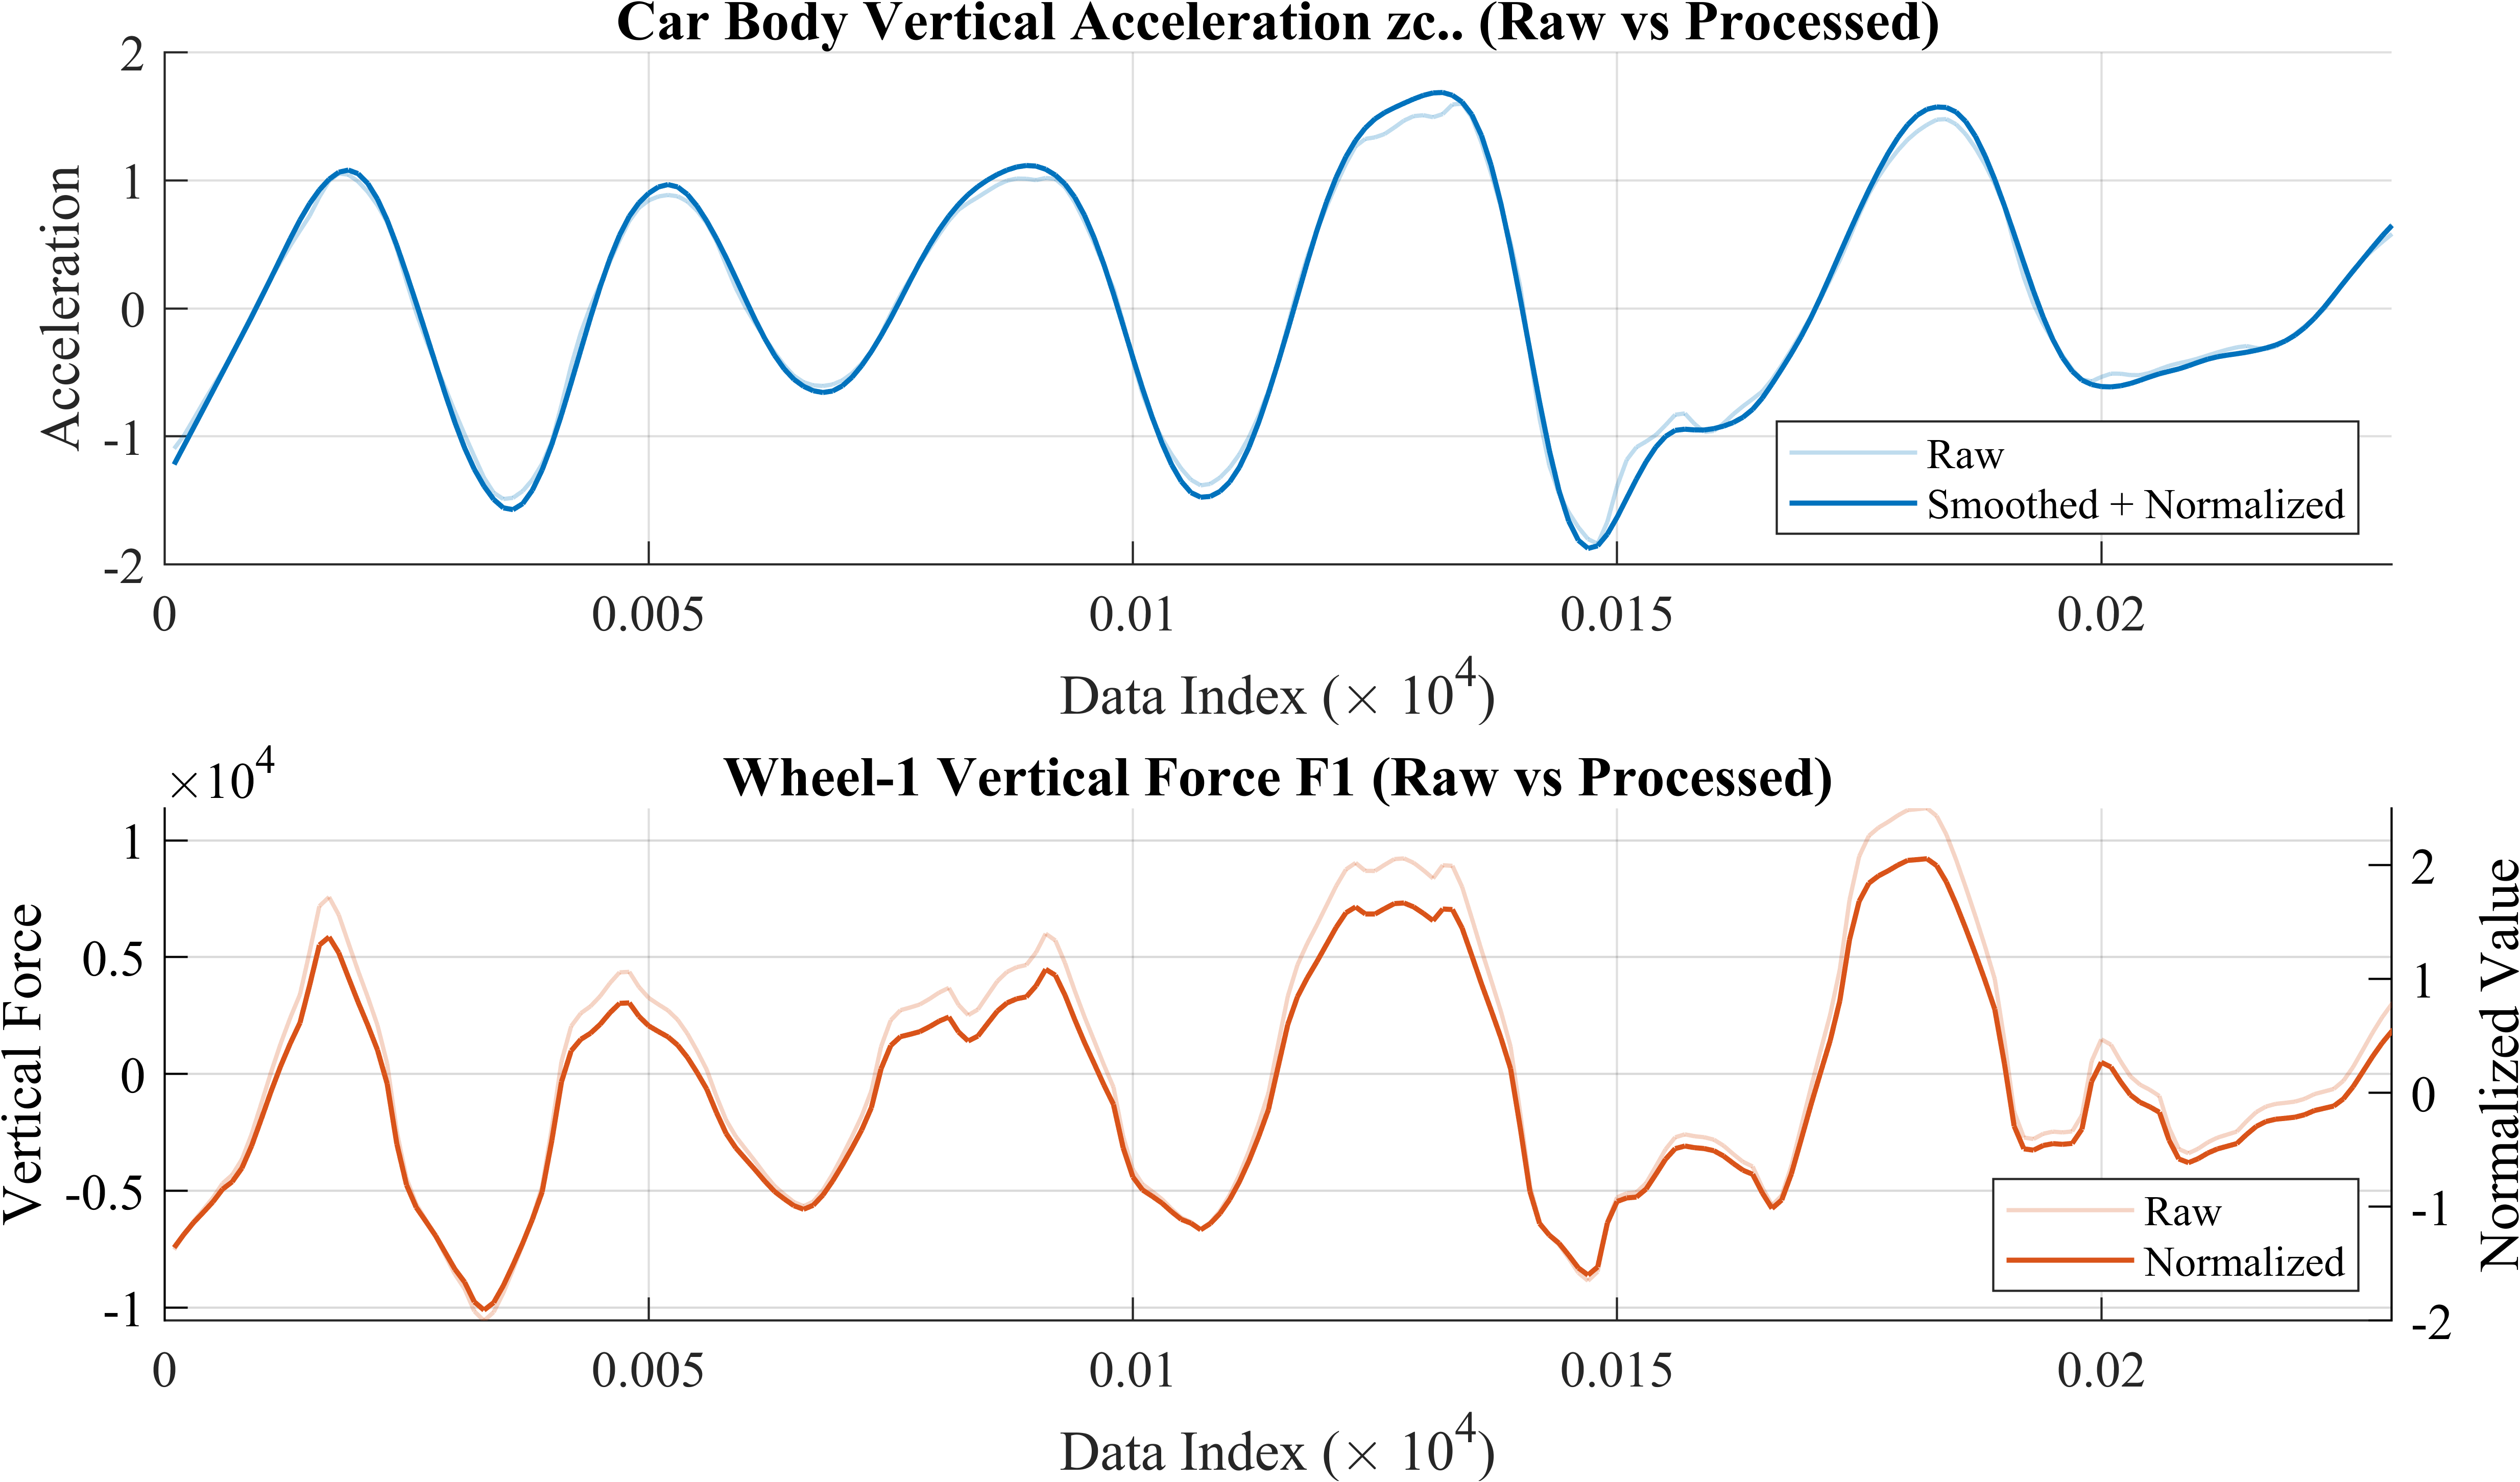
\includegraphics[width=0.65\linewidth]{pics/zc_and_F1_comparison.png}
    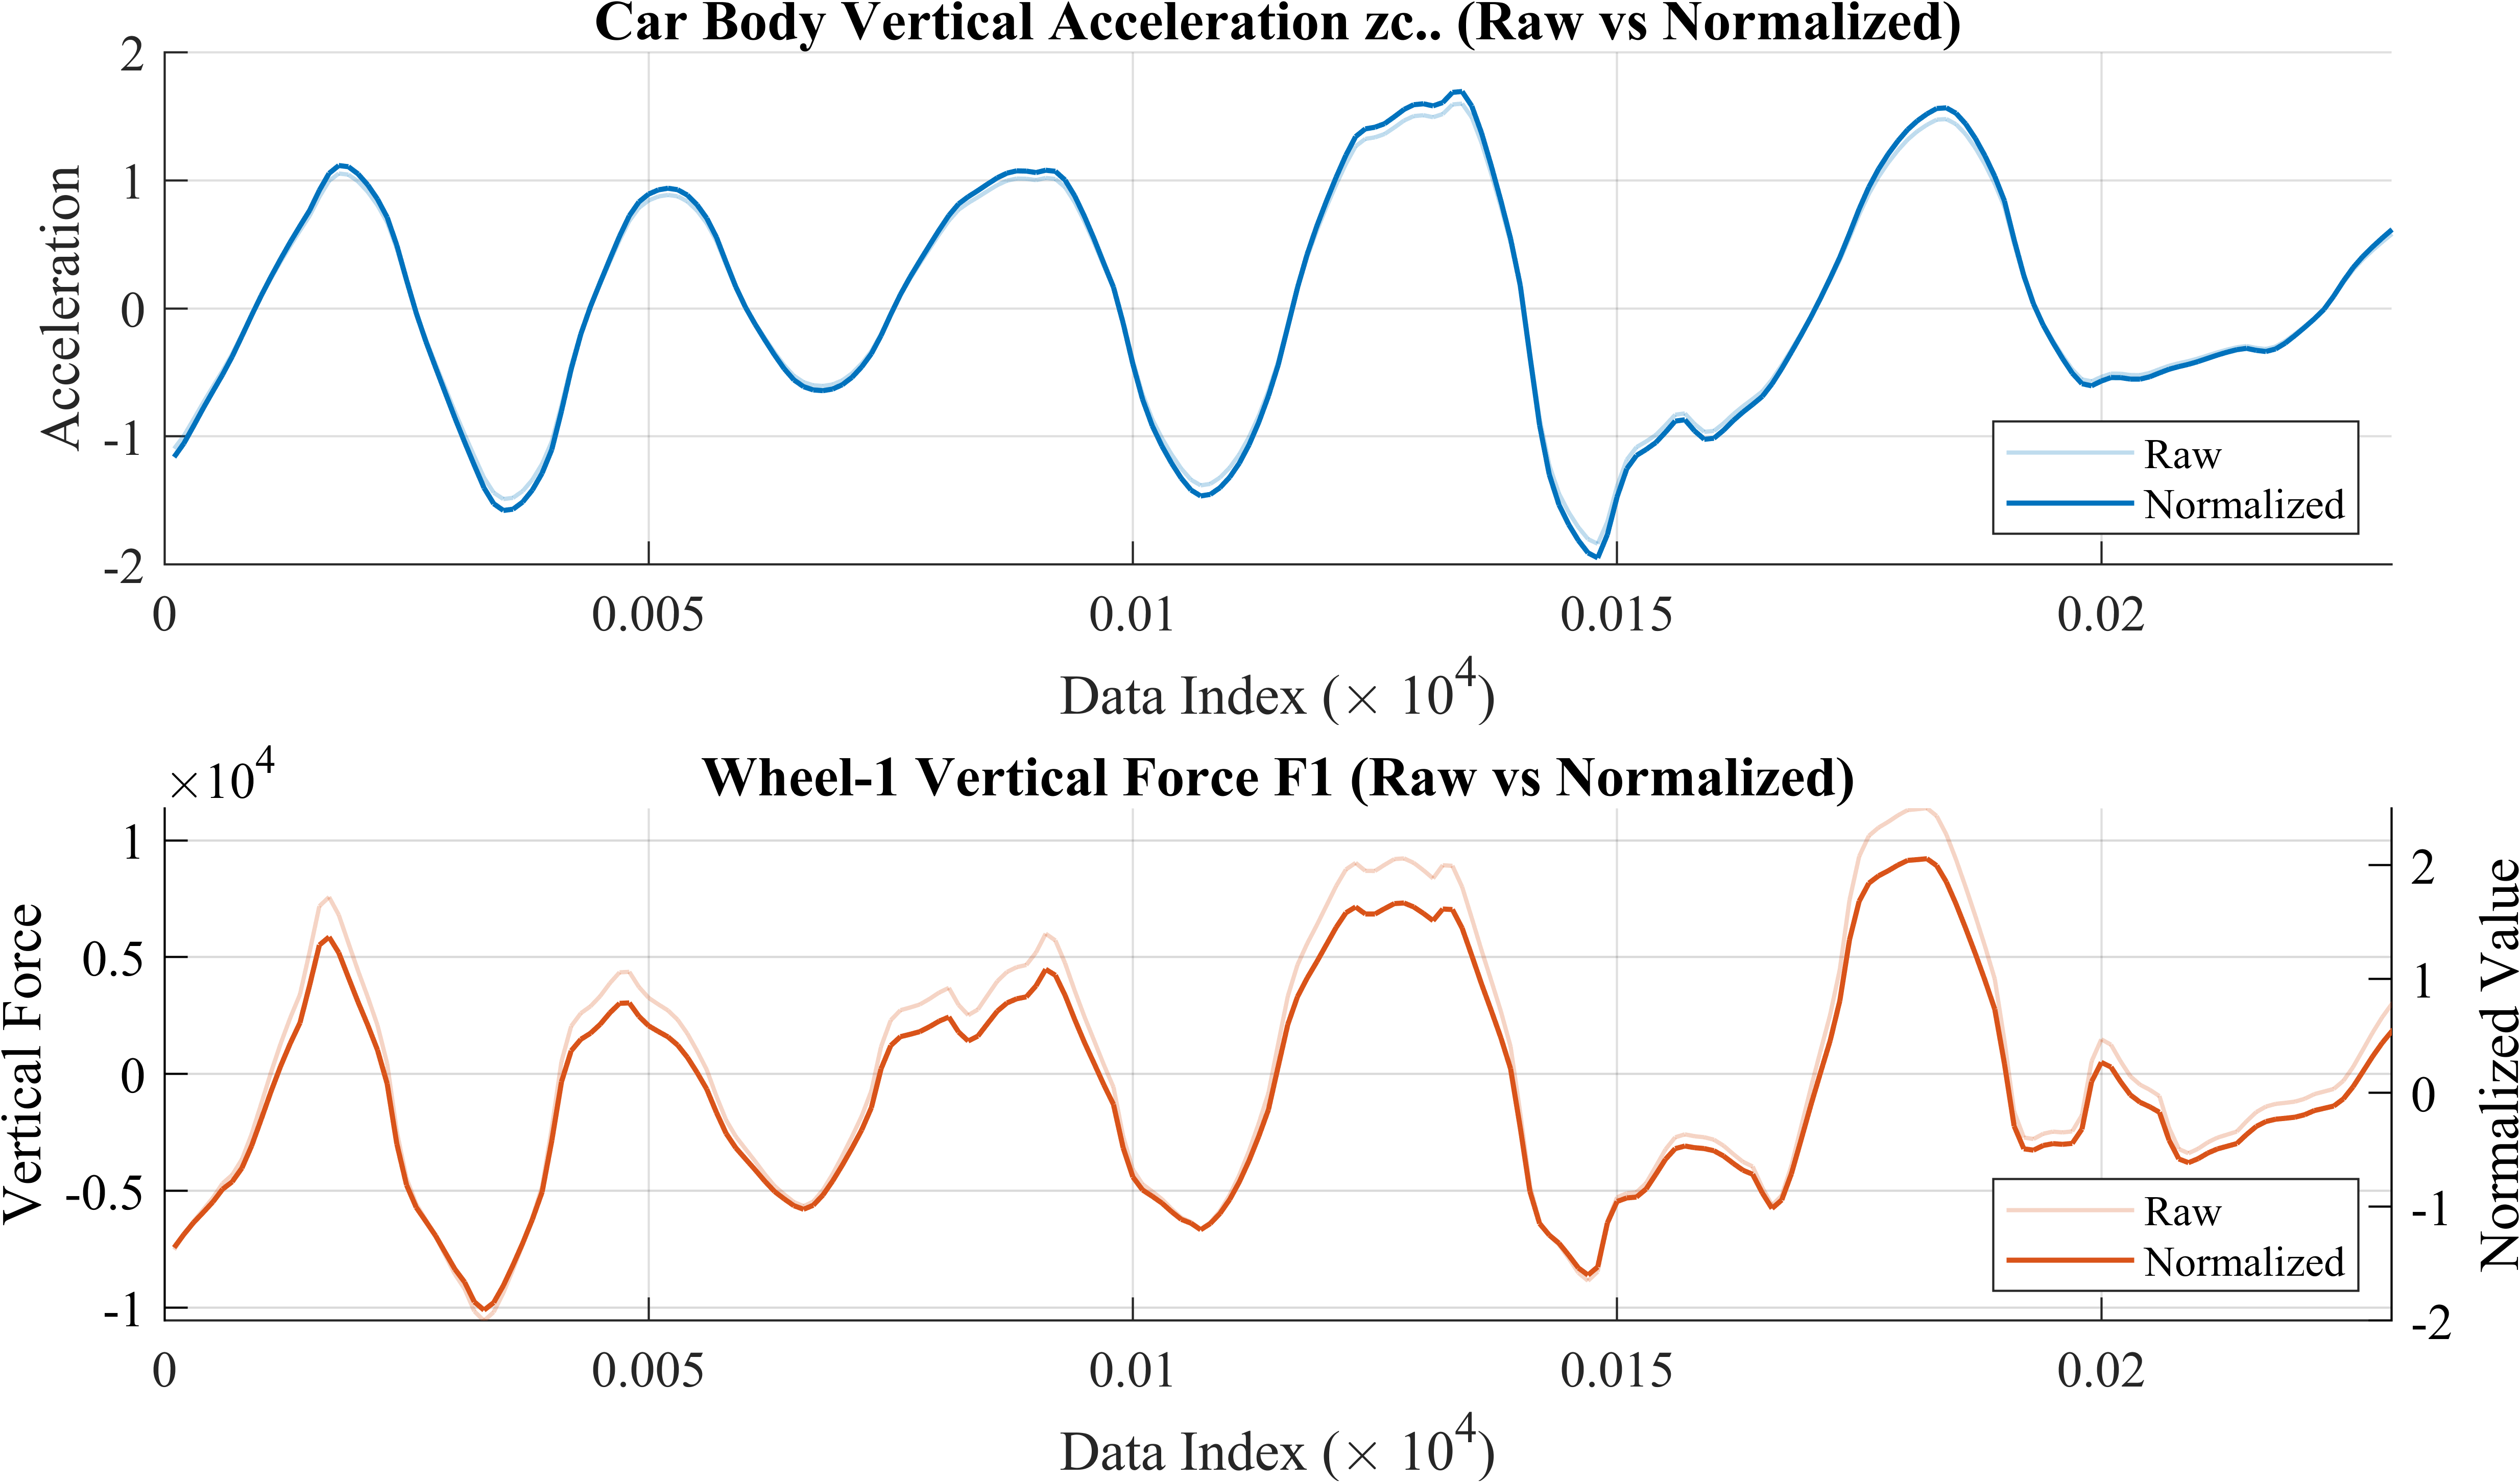
\includegraphics[width=0.65\linewidth]{pics/zc_and_F1_no_smoothing_comparison.png}
    \caption{数据处理前后对比图}
    \vspace{-0.3cm}
\end{figure}
\par{}
\textbf{第2步：选择模型并设计模型结构。}首先按.csv中的分配，定义输入特征与输出标签；接着设置模型参数如下表：
\begin{table}[H]
    \vspace{-0.2cm}
    \centering
    \caption{模型结构参数配置}\label{tab:model_params}
    \vspace{-0.3cm}
    \footnotesize\renewcommand{\arraystretch}{1.15}\begin{tabular}{ccc}
        \specialrule{\heavyrulewidth}{0pt}{0pt}
        \cellcolor{gray!20}参数名称 & \cellcolor{gray!20}程序内参数名 & \cellcolor{gray!20}取值 \\
        \specialrule{\lightrulewidth}{0pt}{0pt}
        时间窗口长度                  & SEQ\_LEN                  & 50                    \\
        输入维度                    & INPUT\_SIZE               & 7                     \\
        输出维度                    & OUTPUT\_SIZE              & 4                     \\
        隐藏层维度                   & HIDDEN\_SIZE              & 64                    \\
        循环层数                    & NUM\_LAYERS               & 2                     \\
        Dropout比例               & DROPOUT                   & 0.2                   \\
        \specialrule{\heavyrulewidth}{0pt}{0pt}
    \end{tabular}
    \vspace{-0.2cm}
\end{table}
\par{}
其中时间窗口长度指的是每次训练取前50个数据点作为样本；输入维度与输出维度就是输入特征与输出标签的数量；隐藏层维度表示 LSTM/GRU 在每个时间步输出 64 维隐藏状态，用于表达输入序列中的动态特征；循环层数设置为 2，表示模型采用两层堆叠的 LSTM/GRU 结构，以增强对时间序列特征的提取能力，同时避免网络过深导致训练困难或过拟合；Dropout比例的目的是训练时随机让一部分神经元暂时失效，不参与本次计算，测试和预测时再全部启用。
\par{}
接着定义模型名称等参数，并检查各参数。
\par{}
\textbf{第3步：模型训练。}设置训练参数如下表：
\begin{table}[H]
    \vspace{-0.2cm}
    \centering
    \caption{训练超参数配置}\label{tab:params}
    \vspace{-0.2cm}
    \footnotesize\renewcommand{\arraystretch}{1.3}\begin{tabular}{cccc}
        \specialrule{\heavyrulewidth}{0pt}{0pt}
        \cellcolor{gray!20}超参数名称 & \cellcolor{gray!20}程序内参数名 & \cellcolor{gray!20}值 & \cellcolor{gray!20}备注 \\
        \specialrule{\lightrulewidth}{0pt}{0pt}
        训练集比例                    & TRAIN\_RATIO              & 70\%                 & 按时间顺序划分               \\
        验证集比例                    & VAL\_RATIO                & 15\%                 & 用于早停和模型选择             \\
        测试集比例                    & TEST\_RATIO               & 15\%                 & 用于最终性能评估              \\
        学习率                      & LEARNING\_RATE            & 0.001                & Adam 优化器初始学习率         \\
        最大训练轮数                   & MAX\_EPOCHS               & 100                  & 训练上限                  \\
        早停耐心值                    & PATIENCE                  & 10                   & 验证损失连续不下降的最大轮数        \\
        批量大小                     & BATCH\_SIZE               & 32                   & 每批训练样本数               \\
        权重衰减                     & WEIGHT\_DECAY             & 1e-5                 & L2 正则化系数              \\
        优化器                      & optimizer                 & Adam                 & 自适应梯度优化器              \\
        \specialrule{\heavyrulewidth}{0pt}{0pt}
    \end{tabular}
    \vspace{-0.2cm}
\end{table}
\par{}
其中按时间序列的先后顺序将原数据集划分成训练集、验证集与测试集，其中前两者在训练时生效，测试集只在最终预测时生效，进行独立测试集评估，以对模型进行简单的泛化性能测试，但严格意义上不算迁移学习；同时对于两种前处理结果的两种模型均展开训练，以便后续对比；再保存模型权重到.pt文件，保存训练损失等过程信息到.csv文件。
\par{}
\textbf{第4步：迁移学习。}加载平滑+归一化数据上训练得到的LSTM与GRU权重，并将其作为预训练权重迁移到仅归一化数据上继续训练，从而观察模型在不同数据分布之间迁移后的性能变化。
\par{}
\textbf{第5步：模型评估。}加载普通训练模型与迁移学习模型的最优权重并在测试集上预测，计算MSE、RMSE、MAE等，保存在.csv中并对训练与测试过程中的关键指标进行可视化处理。
\par{}
\textbf{当然还有一个总控脚本，}该脚本按顺序运行第1至5步，报错则停止运行；同时如果检测到存在已完成的步骤，会直接跳过该步骤，直接执行后续步骤。
\par{}
\quad{}
\par{}
\section{实验结果与分析}
\subsection{数据预处理方法对比}
\par{}
本次实验进行了两套预处理：输入特征Savitzky-Golay平滑+Z-score标准化，输出标签仅Z-score标准化；输入特征与输出标签仅Z-score标准化。
\par{}
如图2，这是两种模型在两套预处理方法下得出的的预测结果波形图片段，每种情况选了4个片段进行展示，可目测得出在同一模型结果图像的部分尖峰附近，同时对输入进行平滑与归一化处理所得预测图线与实际图线的吻合程度不如只进行归一化处理所得。虽然这不足以量化说明其具体差异，但已经能推测大致结果。
\begin{figure}[H]
    \centering
    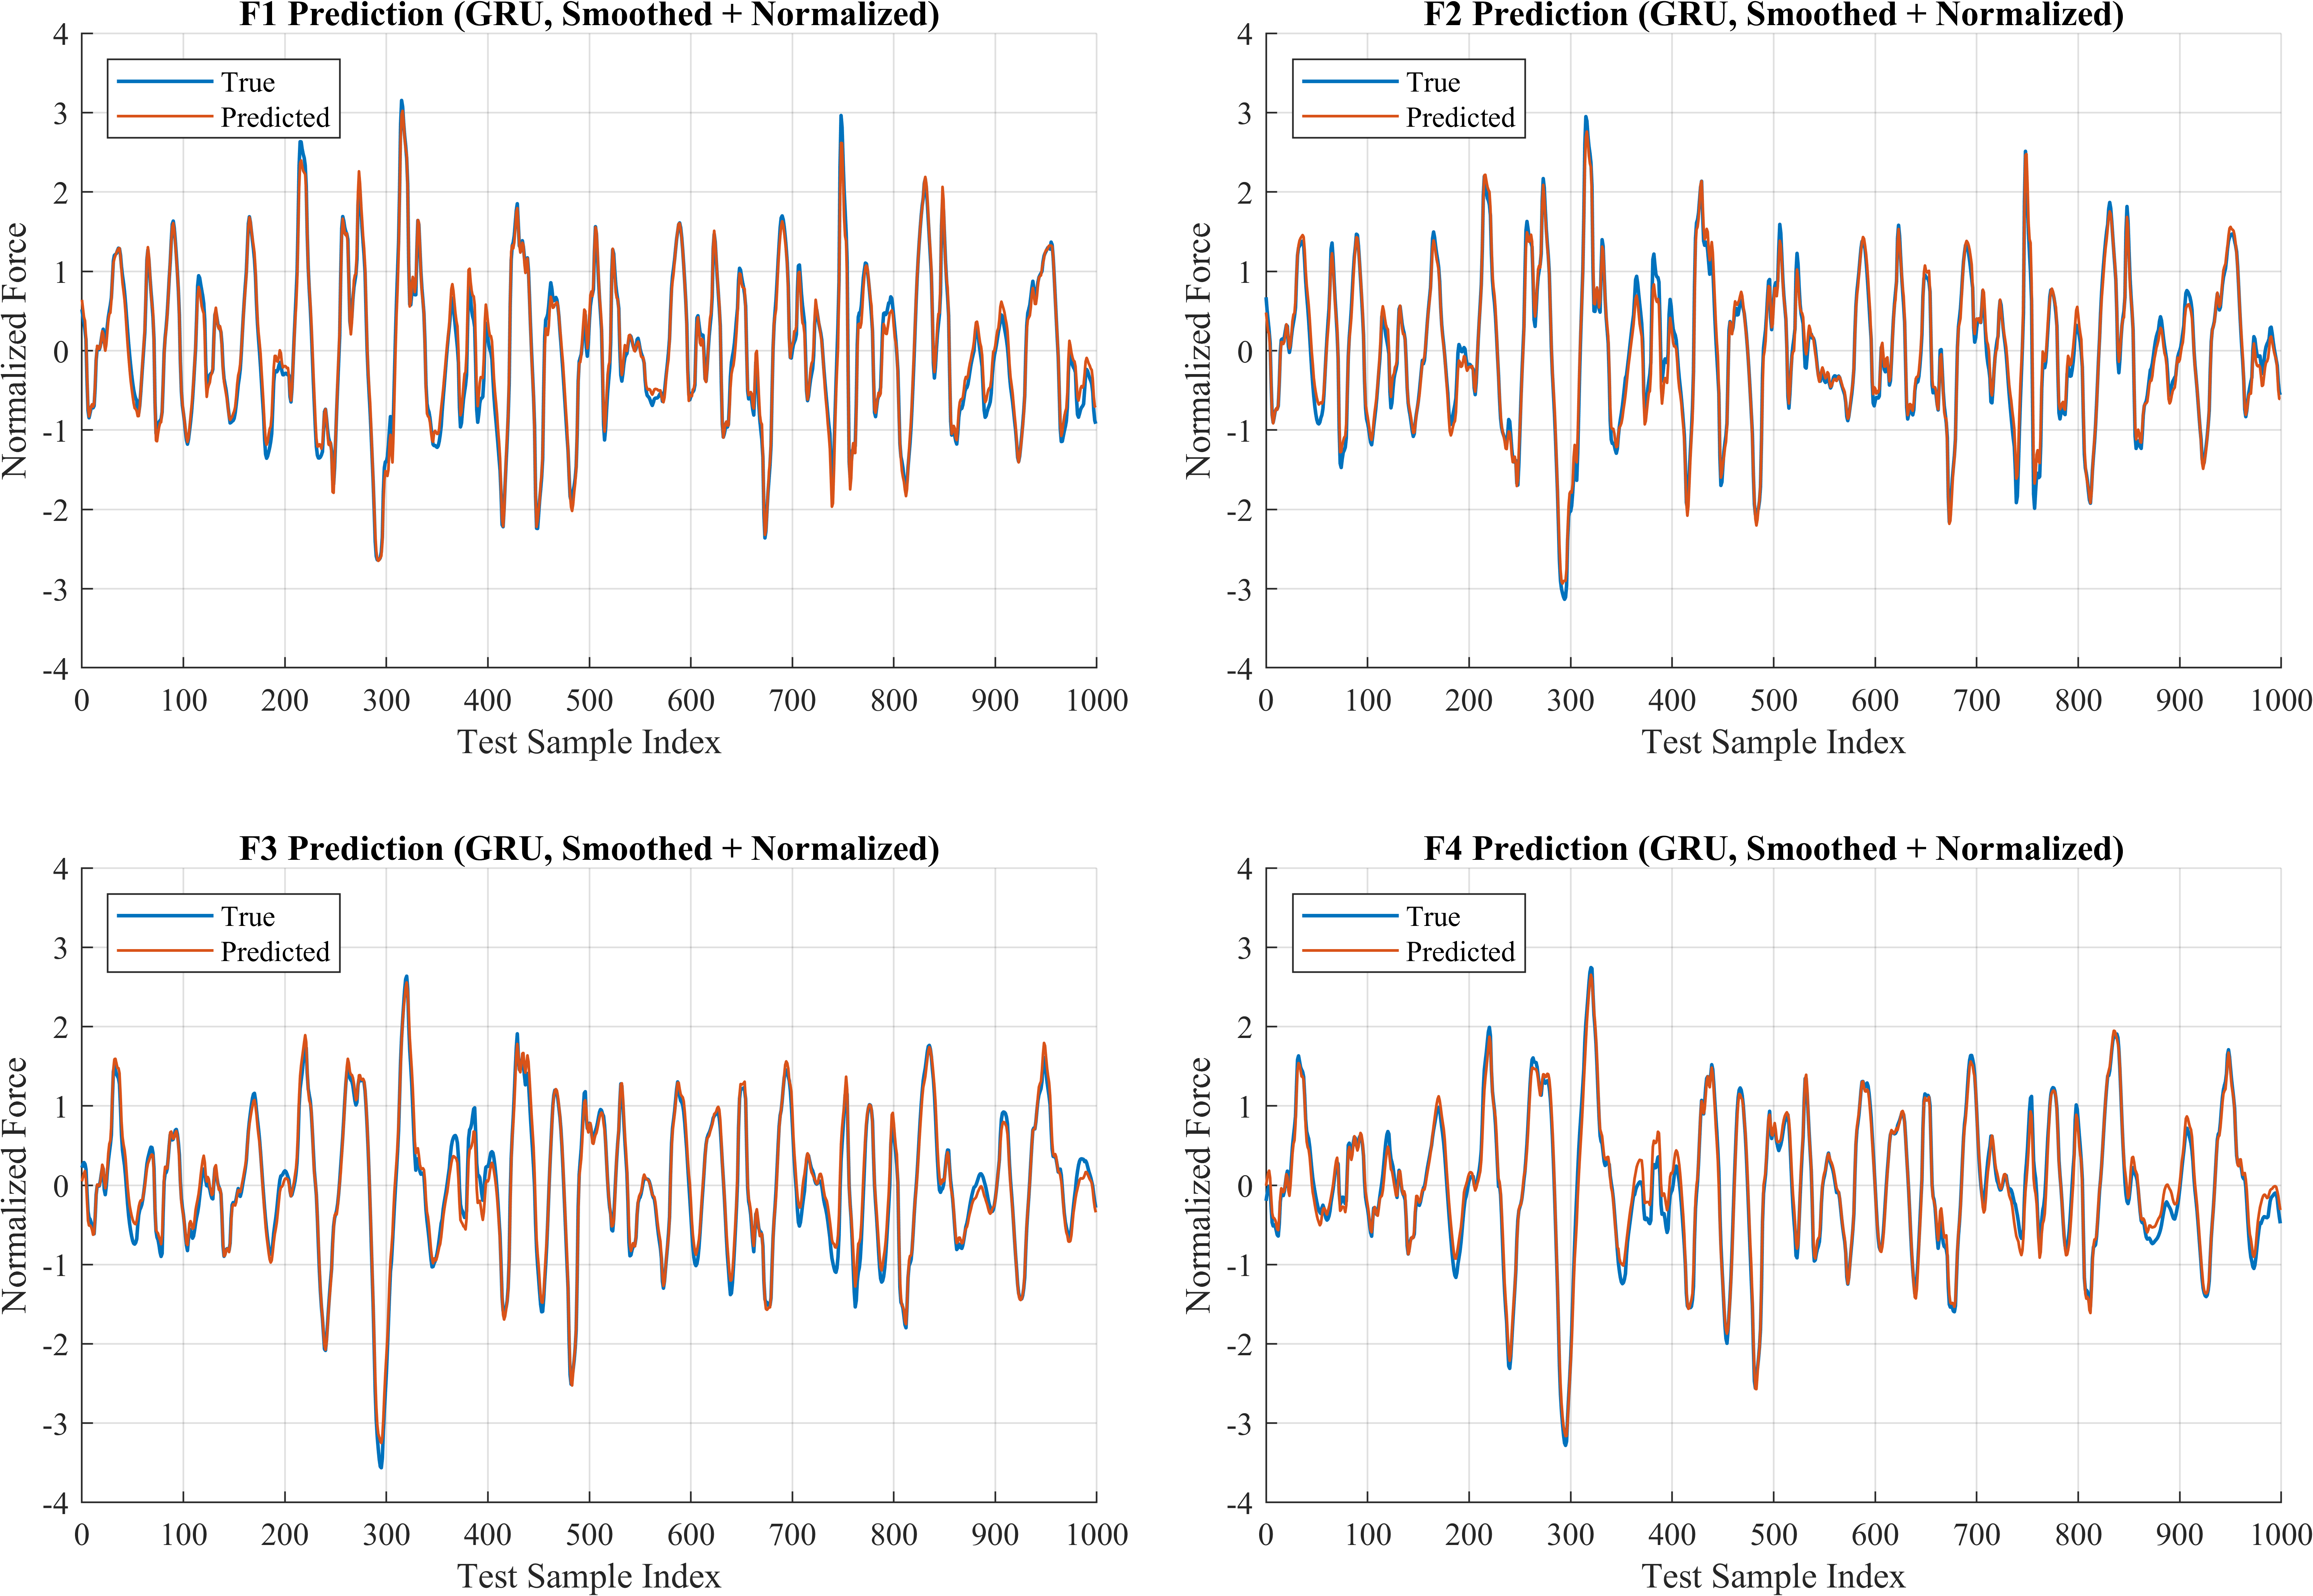
\includegraphics[width=0.48\linewidth]{pics/prediction_comparison_GRU.png}
    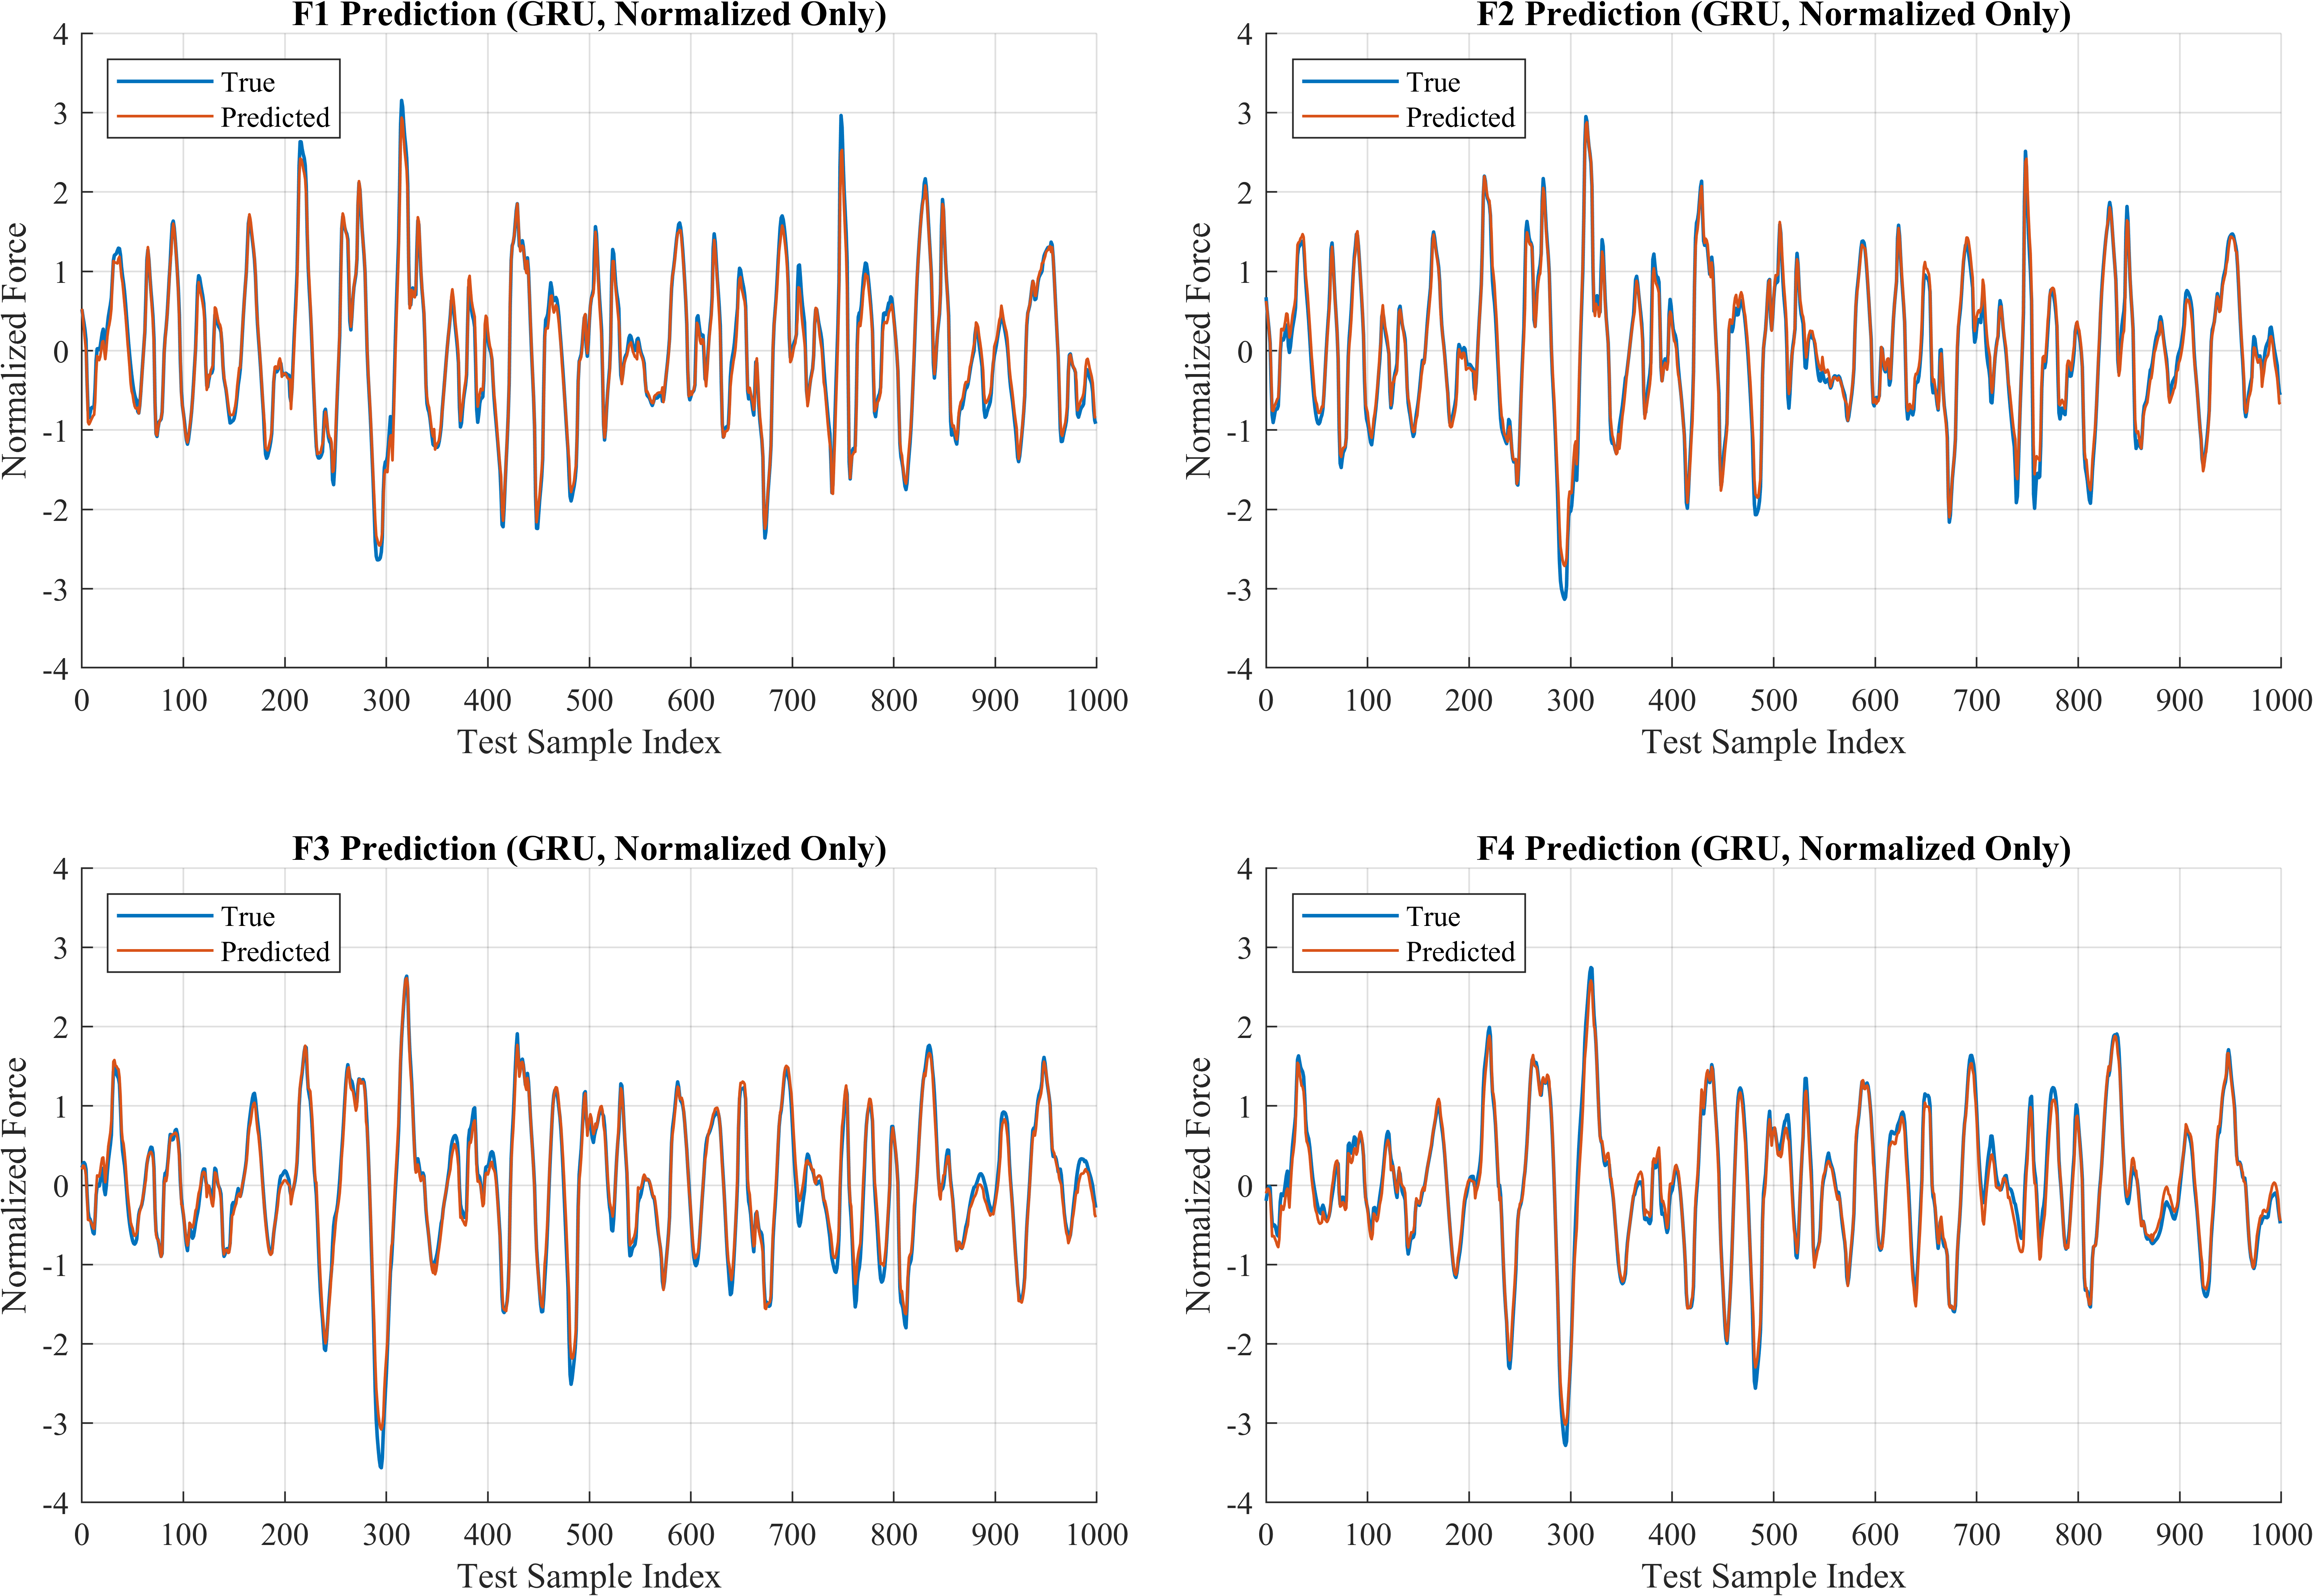
\includegraphics[width=0.48\linewidth]{pics/prediction_comparison_GRU_no_smoothing.png}
    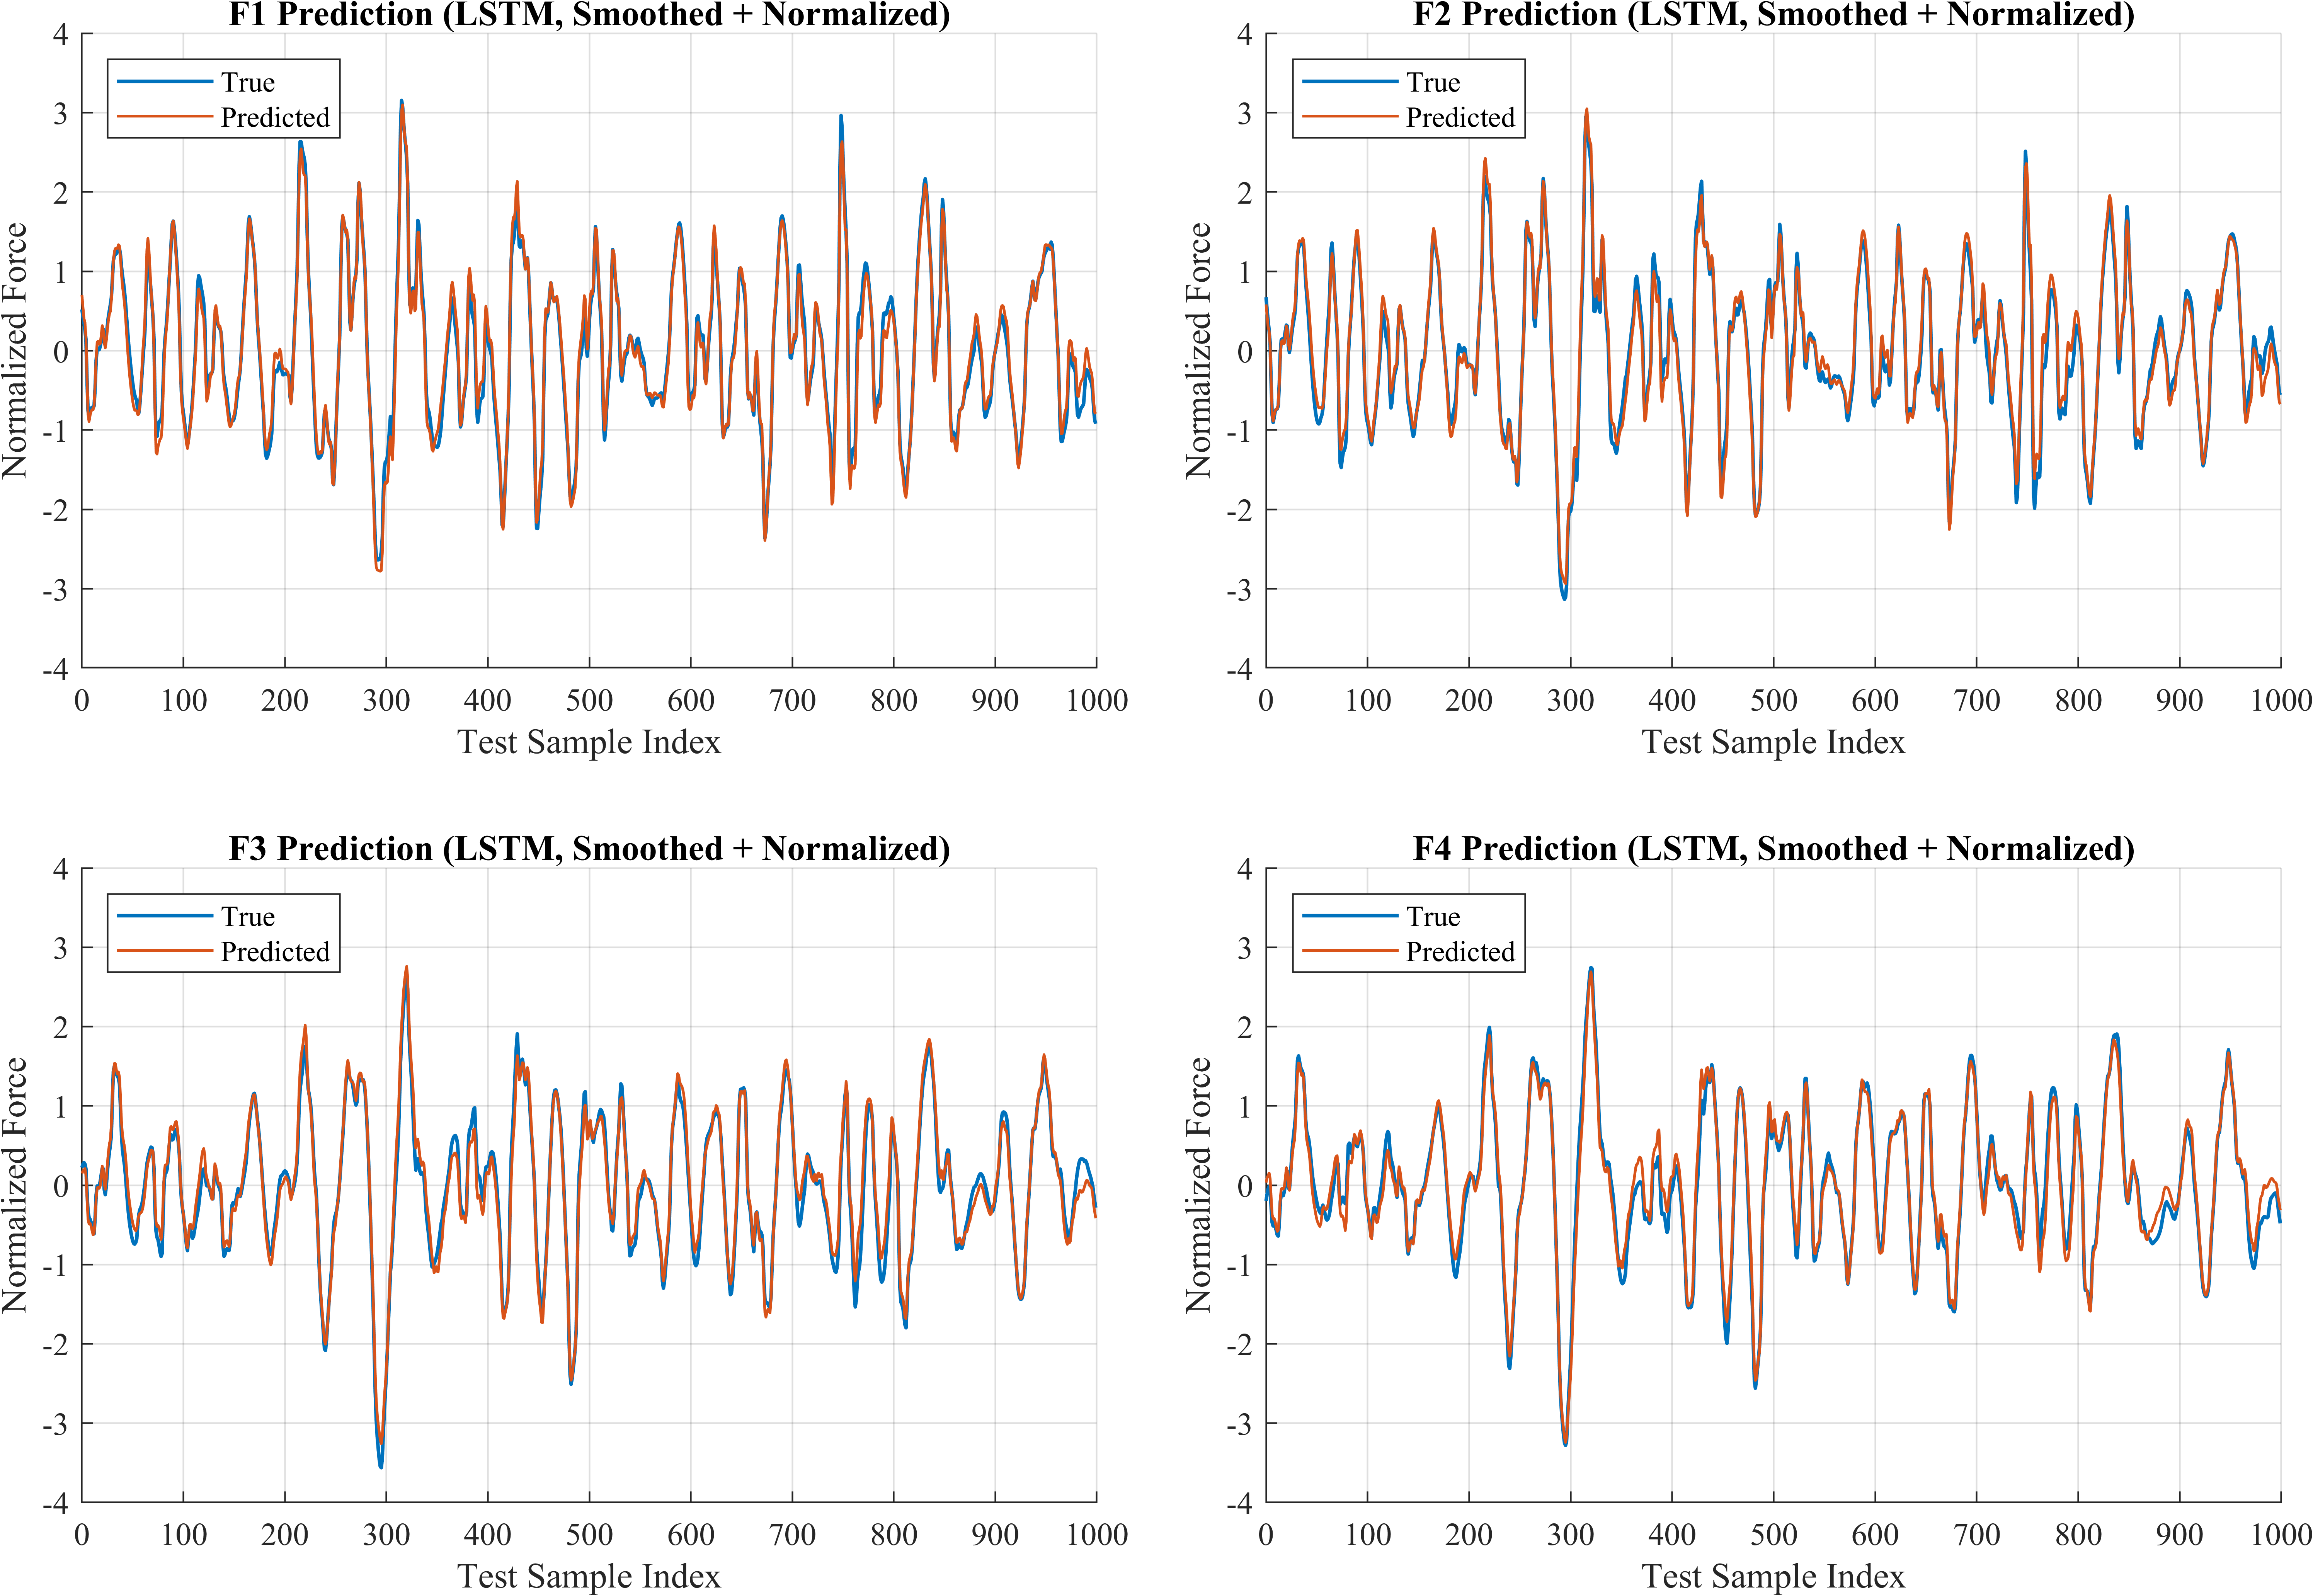
\includegraphics[width=0.48\linewidth]{pics/prediction_comparison_LSTM.png}
    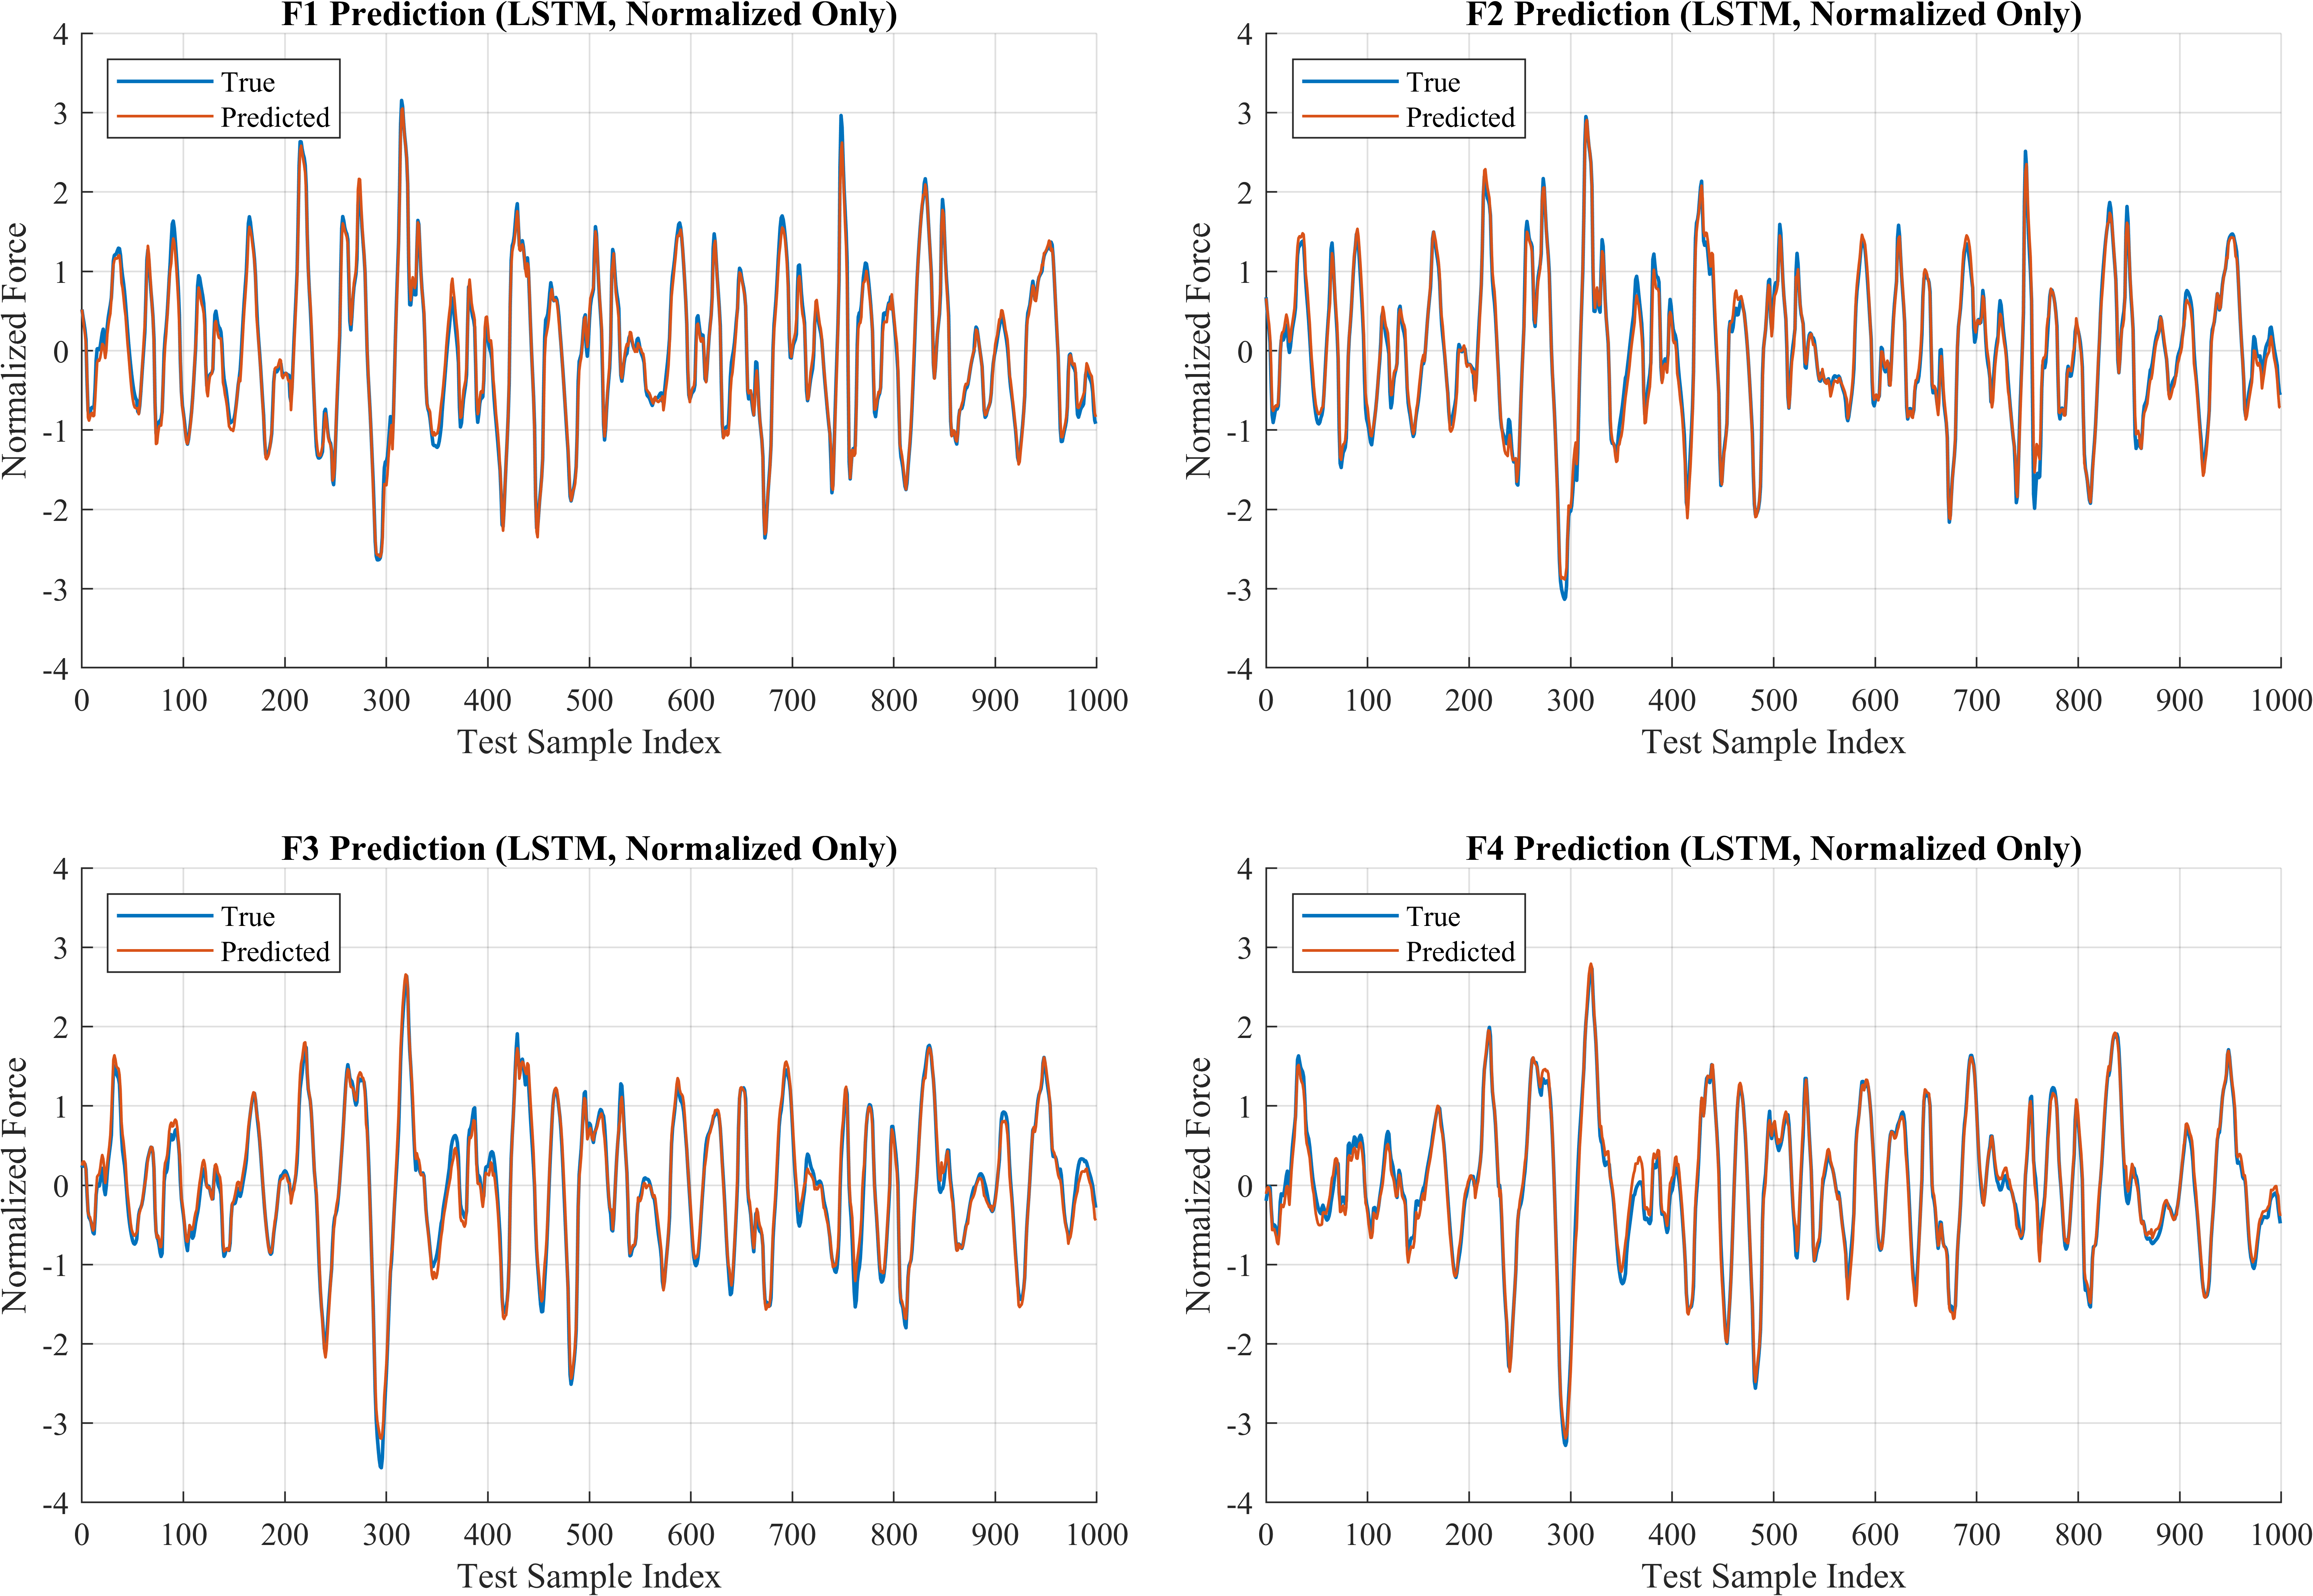
\includegraphics[width=0.48\linewidth]{pics/prediction_comparison_LSTM_no_smoothing.png}
    \caption{测试结果示意图}
    \vspace{-0.5cm}
\end{figure}
\par{}
如图3，这是训练的损失曲线，可得同一模型下仍然是后一种处理方式的训练损失更低，同时训练轮次也更多，意味着此时模型的训练优化性能较好，至于会不会造成过拟合等不利影响，则应当观察图4。
\begin{figure}[H]
    \centering
    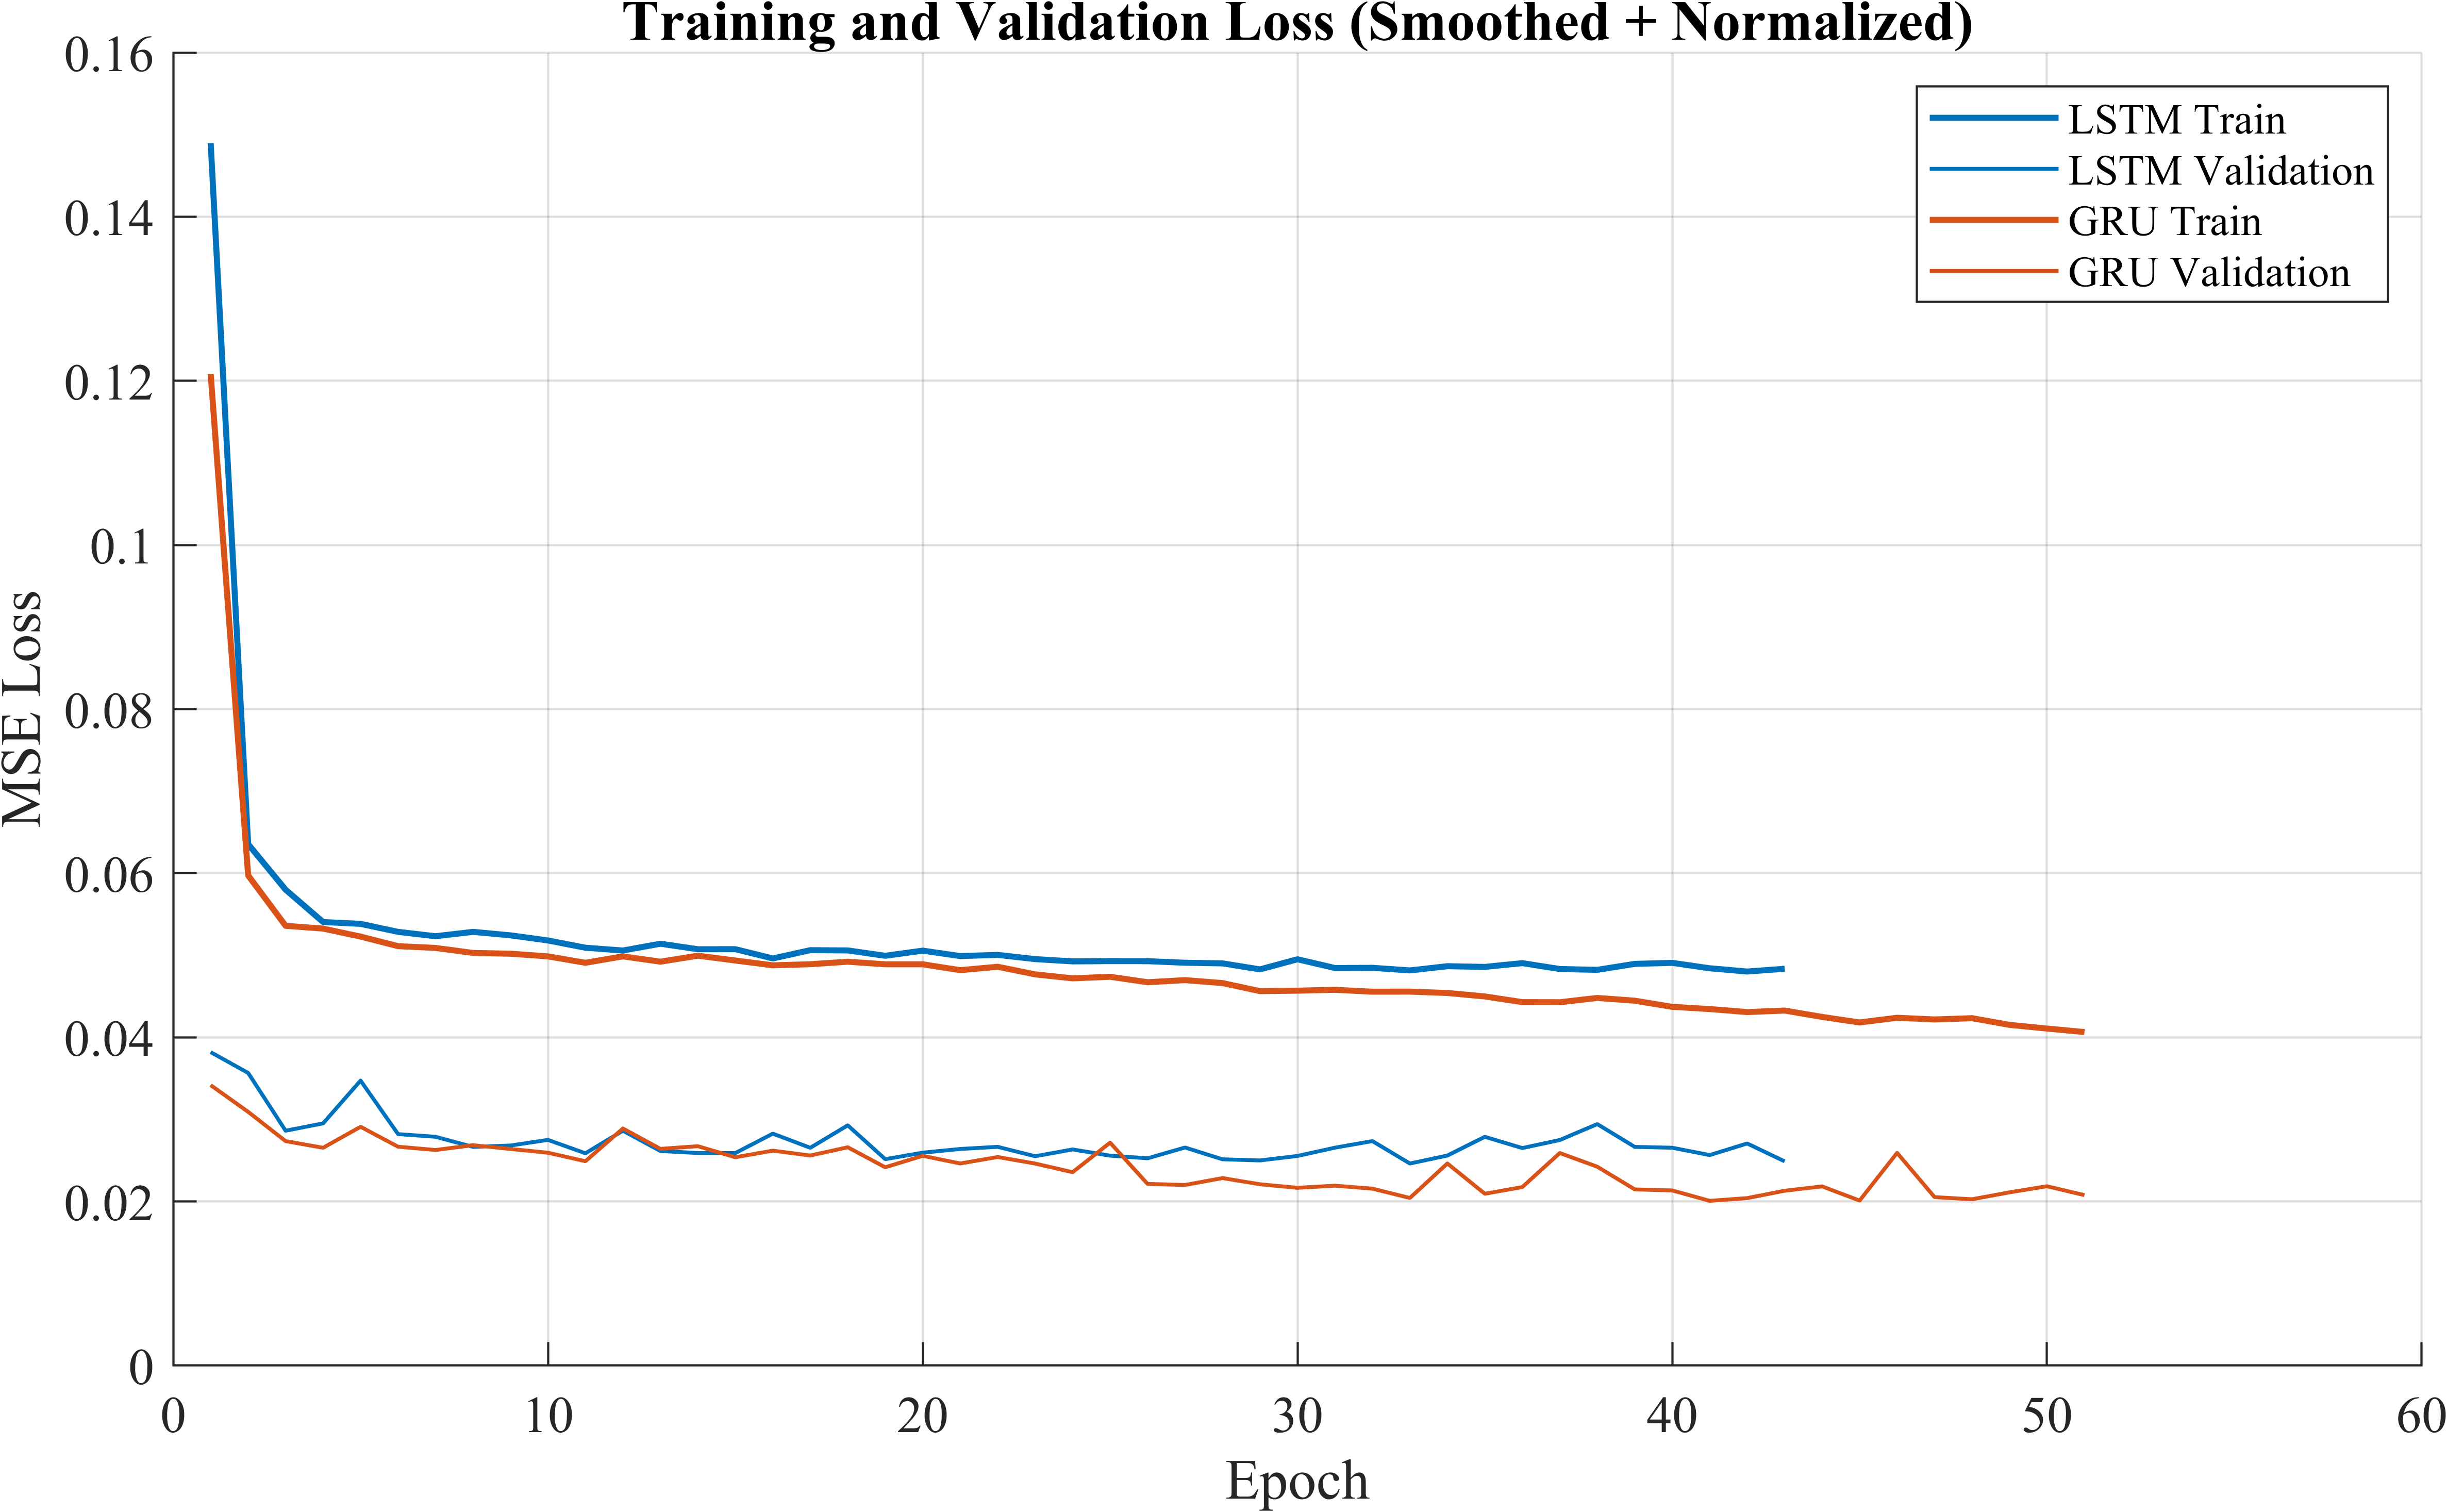
\includegraphics[width=0.8\linewidth]{pics/loss_curve.png}
    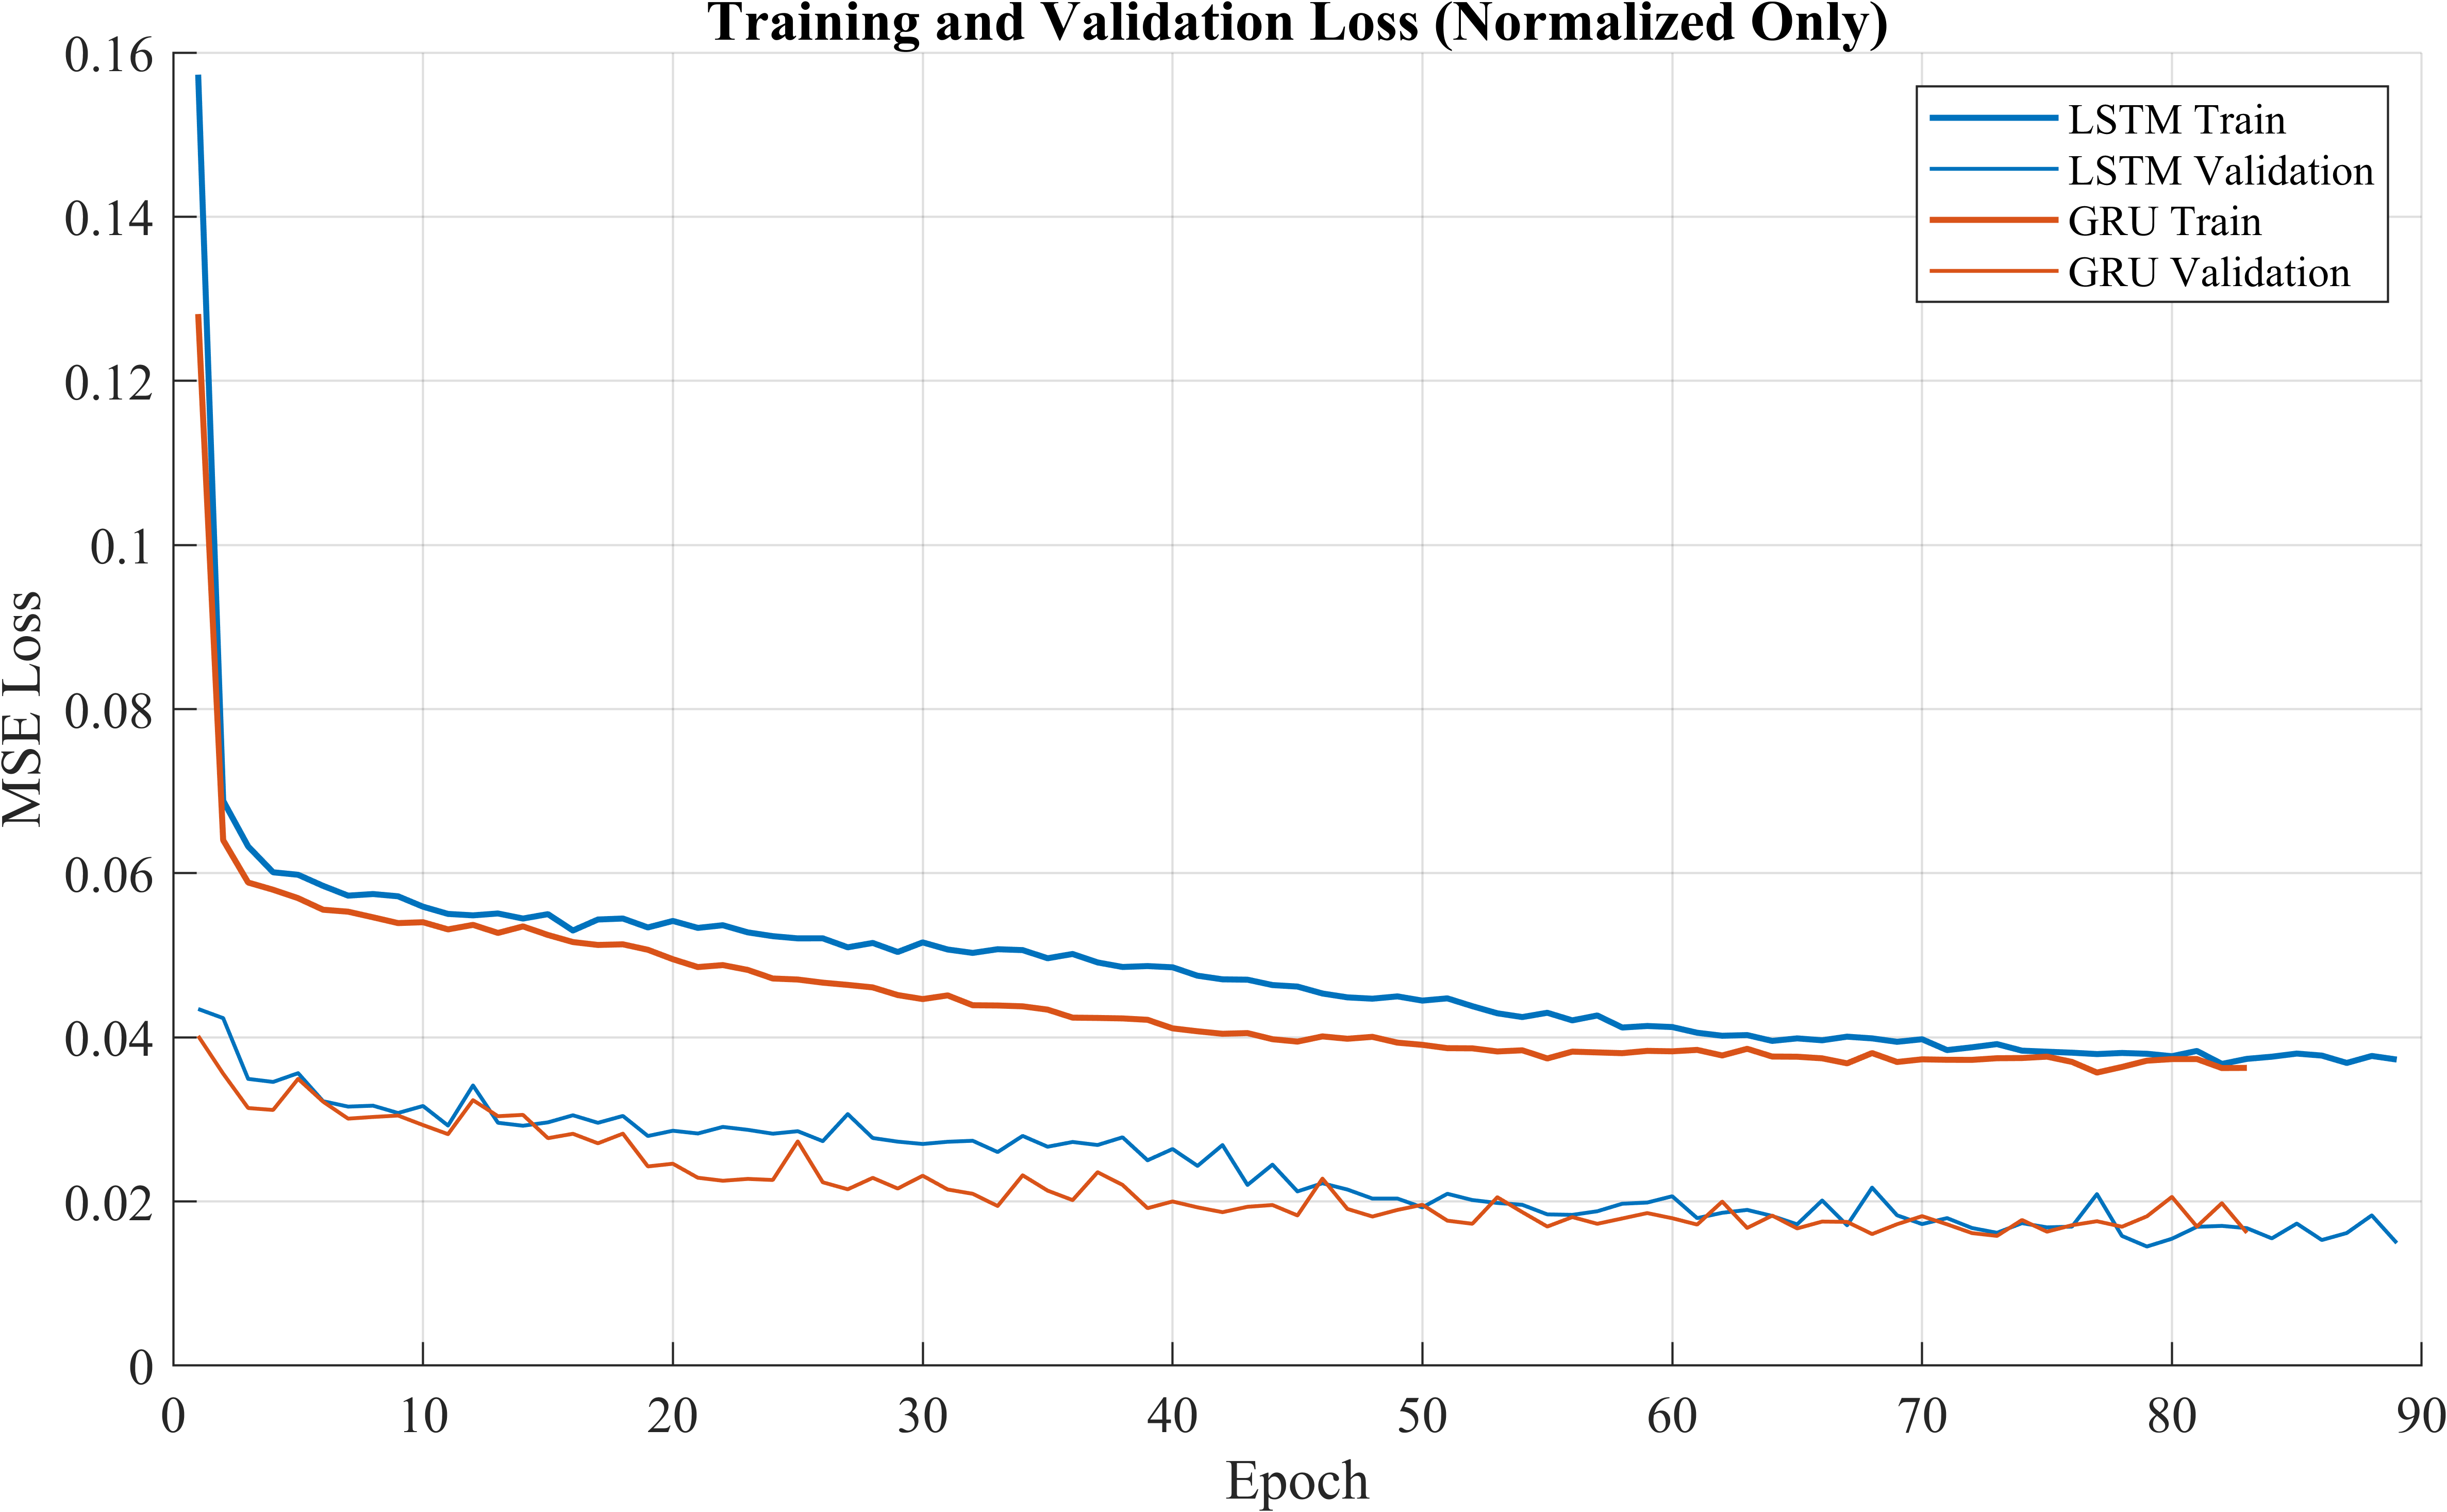
\includegraphics[width=0.8\linewidth]{pics/loss_curve_no_smoothing.png}
    \caption{损失曲线对比}
    \vspace{-0.5cm}
\end{figure}
\par{}
图4为两种处理方法的总体指标对比，可见MSE、RMSE与MAE这几个关键指标都是仅归一化处理时更低。由公式
\begin{align*}
    \mathrm{MSE}  & =\frac{1}{n}\sum_{i=1}^{n}(y_i-\hat{y}_i)^2        \\
    \mathrm{RMSE} & =\sqrt{\frac{1}{n}\sum_{i=1}^{n}(y_i-\hat{y}_i)^2} \\
    \mathrm{MAE}  & =\frac{1}{n}\sum_{i=1}^{n}|y_i-\hat{y}_i|
\end{align*}
可得，只需要关注RMSE与MAE即可，RMSE指均方根误差、MAE指平均绝对误差，前者对预测误差的某些较大值更加敏感，主要反映误差的离散程度；后者对异常大误差的敏感性较低，主要反映平均误差。因此，仅归一化的处理方法下的结果从误差的均值与离散度上都更优前一种；这也说明后一种处理方法带来的训练轮次增加并不会造成过拟合现象，反而会让测试集表现效果更好。
\par{}
这也说明当前算例中Savitzky-Golay平滑虽然能降低输入噪声，但也可能削弱了车辆振动信号中的局部峰值和快速变化信息；而这些快速变化可能对车轮垂向力预测有用。因此针对该数据集，保留原始输入动态细节比额外平滑更有利。
\begin{figure}[H]
    \centering
    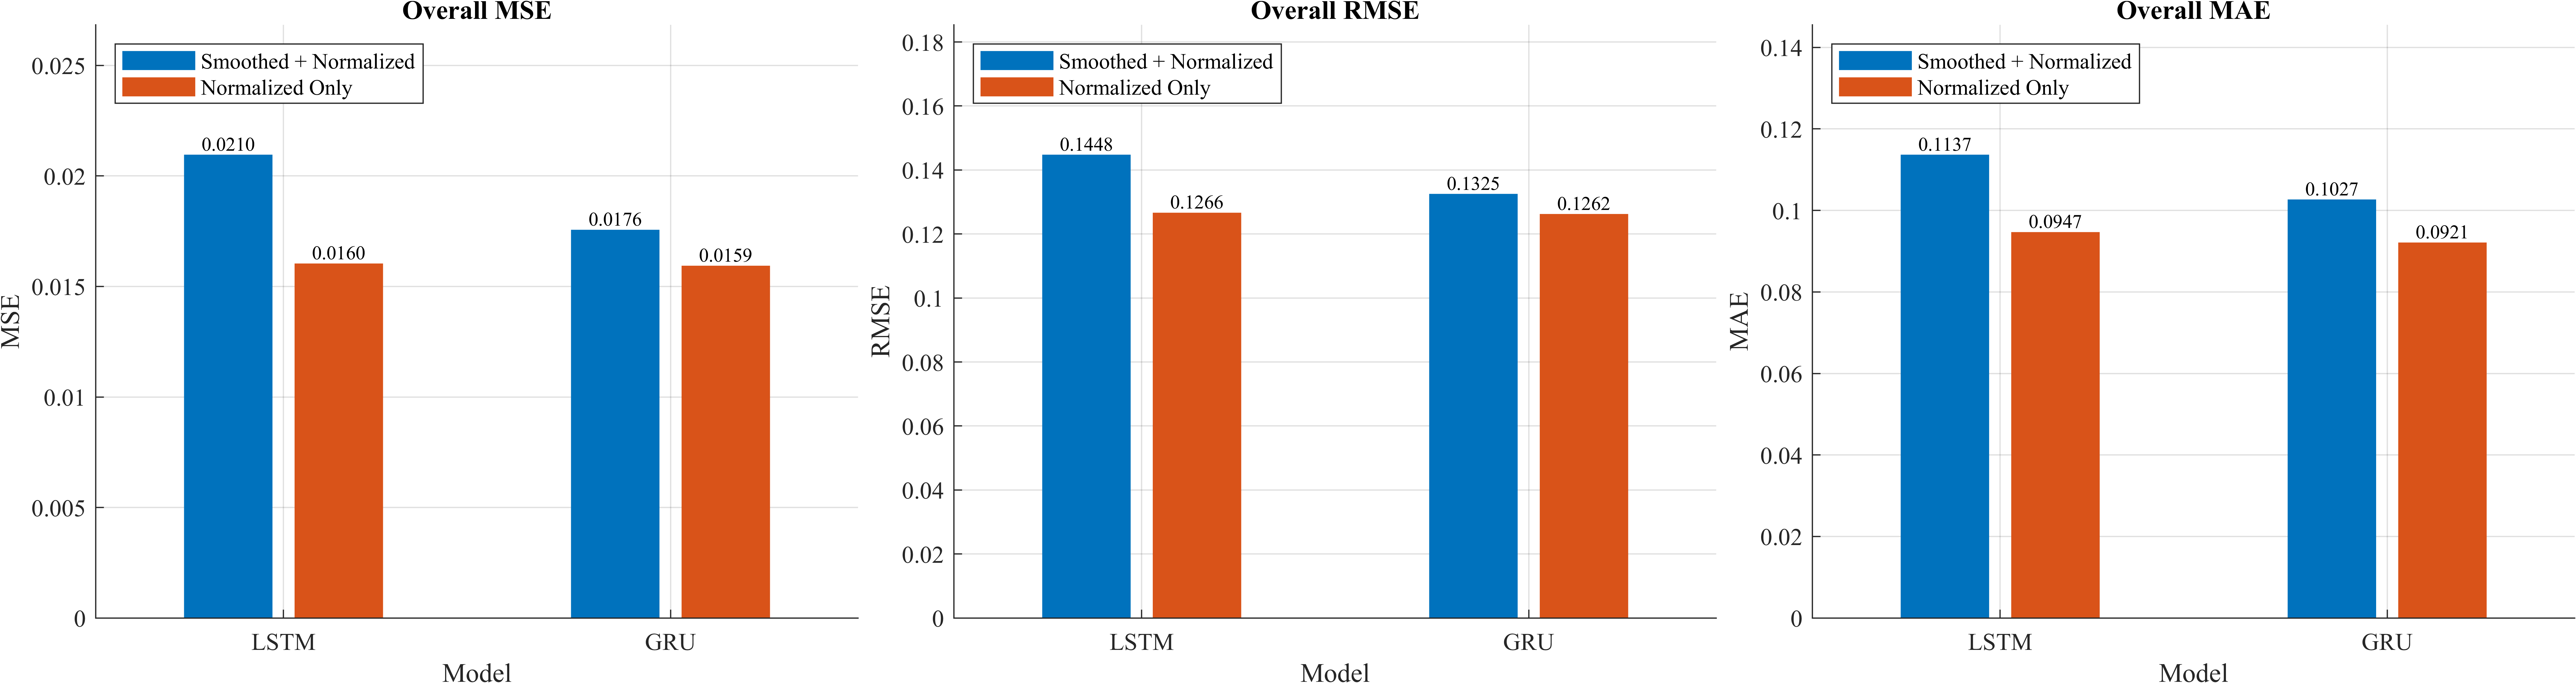
\includegraphics[width=0.98\linewidth]{pics/preprocessing_metrics_comparison.png}
    \caption{两种处理方法各项总体指标对比}
    \vspace{-0.5cm}
\end{figure}
\vspace{0.25cm}
\subsection{网络/模型对比}
\par{}
由超参数表得，两种模型的网络结构基本一致，区别主要还是在前文中所说的门控结构；从第二步输出的可训练参数数量得，GRU的参数少于LSTM，更为轻量化，也符合前面对门控结构复杂度的分析。
\par{}
如图3，从训练损失曲线看，同一预处理方案下的GRU损失曲线基本低于LSTM，因此对于该数据集，训练时GRU的优化性能更好；但GRU的训练轮次比LSTM略多，是因为早停参数设置使得LSTM较早进入验证损失停滞，而GRU在较长时间内仍能继续改善验证损失；从下文分析的测试指标看，GRU的额外训练轮次并未造成明显过拟合，反而对应更好的预测性能。
\begin{figure}[H]
    \centering
    
\includegraphics[width=0.98\linewidth]{pics/metrics_comparison.png}
    
\includegraphics[width=0.98\linewidth]{pics/metrics_comparison_no_smoothing.png}
    \caption{两种模型各项指标对比}
    \vspace{-0.5cm}
\end{figure}
\par{}
如图5，从测试集指标来看，GRU在同种预处理方案下绝大多数指标都优于LSTM，尤其是同时进行了平滑+归一化的数据上，两者RMSE与MAE相差更明显，说明在经平滑后的输入信号中，GRU 的门控结构已经足够提取主要时序特征，而且参数量更少，训练更稳定；而在仅归一化的结果上，GRU的RMSE与MAE仍然略小于LSTM，说明二者在整体误差水平上接近，但 GRU 的平均绝对误差略小，预测偏差更稳定一些。
\par{}
该结果的原因可能是GRU参数更少，在当前数据规模和窗口长度下更容易训练稳定，也不容易出现过拟合；而LSTM表达能力更强，但也更依赖充足数据和合适的调参。因此，本算例中的相同模型参数设置下，GRU以更简单的门控结构获得了更好的综合预测效果，可作为更优基准模型。
\vspace{0.25cm}
\subsection{迁移学习效果}
\par{}
在迁移学习实验中，LSTM和GRU均加载在平滑+归一化处理后的数据上训练得到的预训练权重，并在“仅归一化”数据上进行再训练，即迁移学习。如图6，训练过程方面，GRU在第43轮停止训练，明显早于LSTM的第88轮，表明GRU的收敛速度更快；但其最佳验证损失和测试误差均高于LSTM。因此，在本实验的迁移学习设置下，GRU 具有训练效率优势，而LSTM具有更好的最终预测精度。
\begin{figure}[H]
    \centering
    \vspace{-0.2cm}
    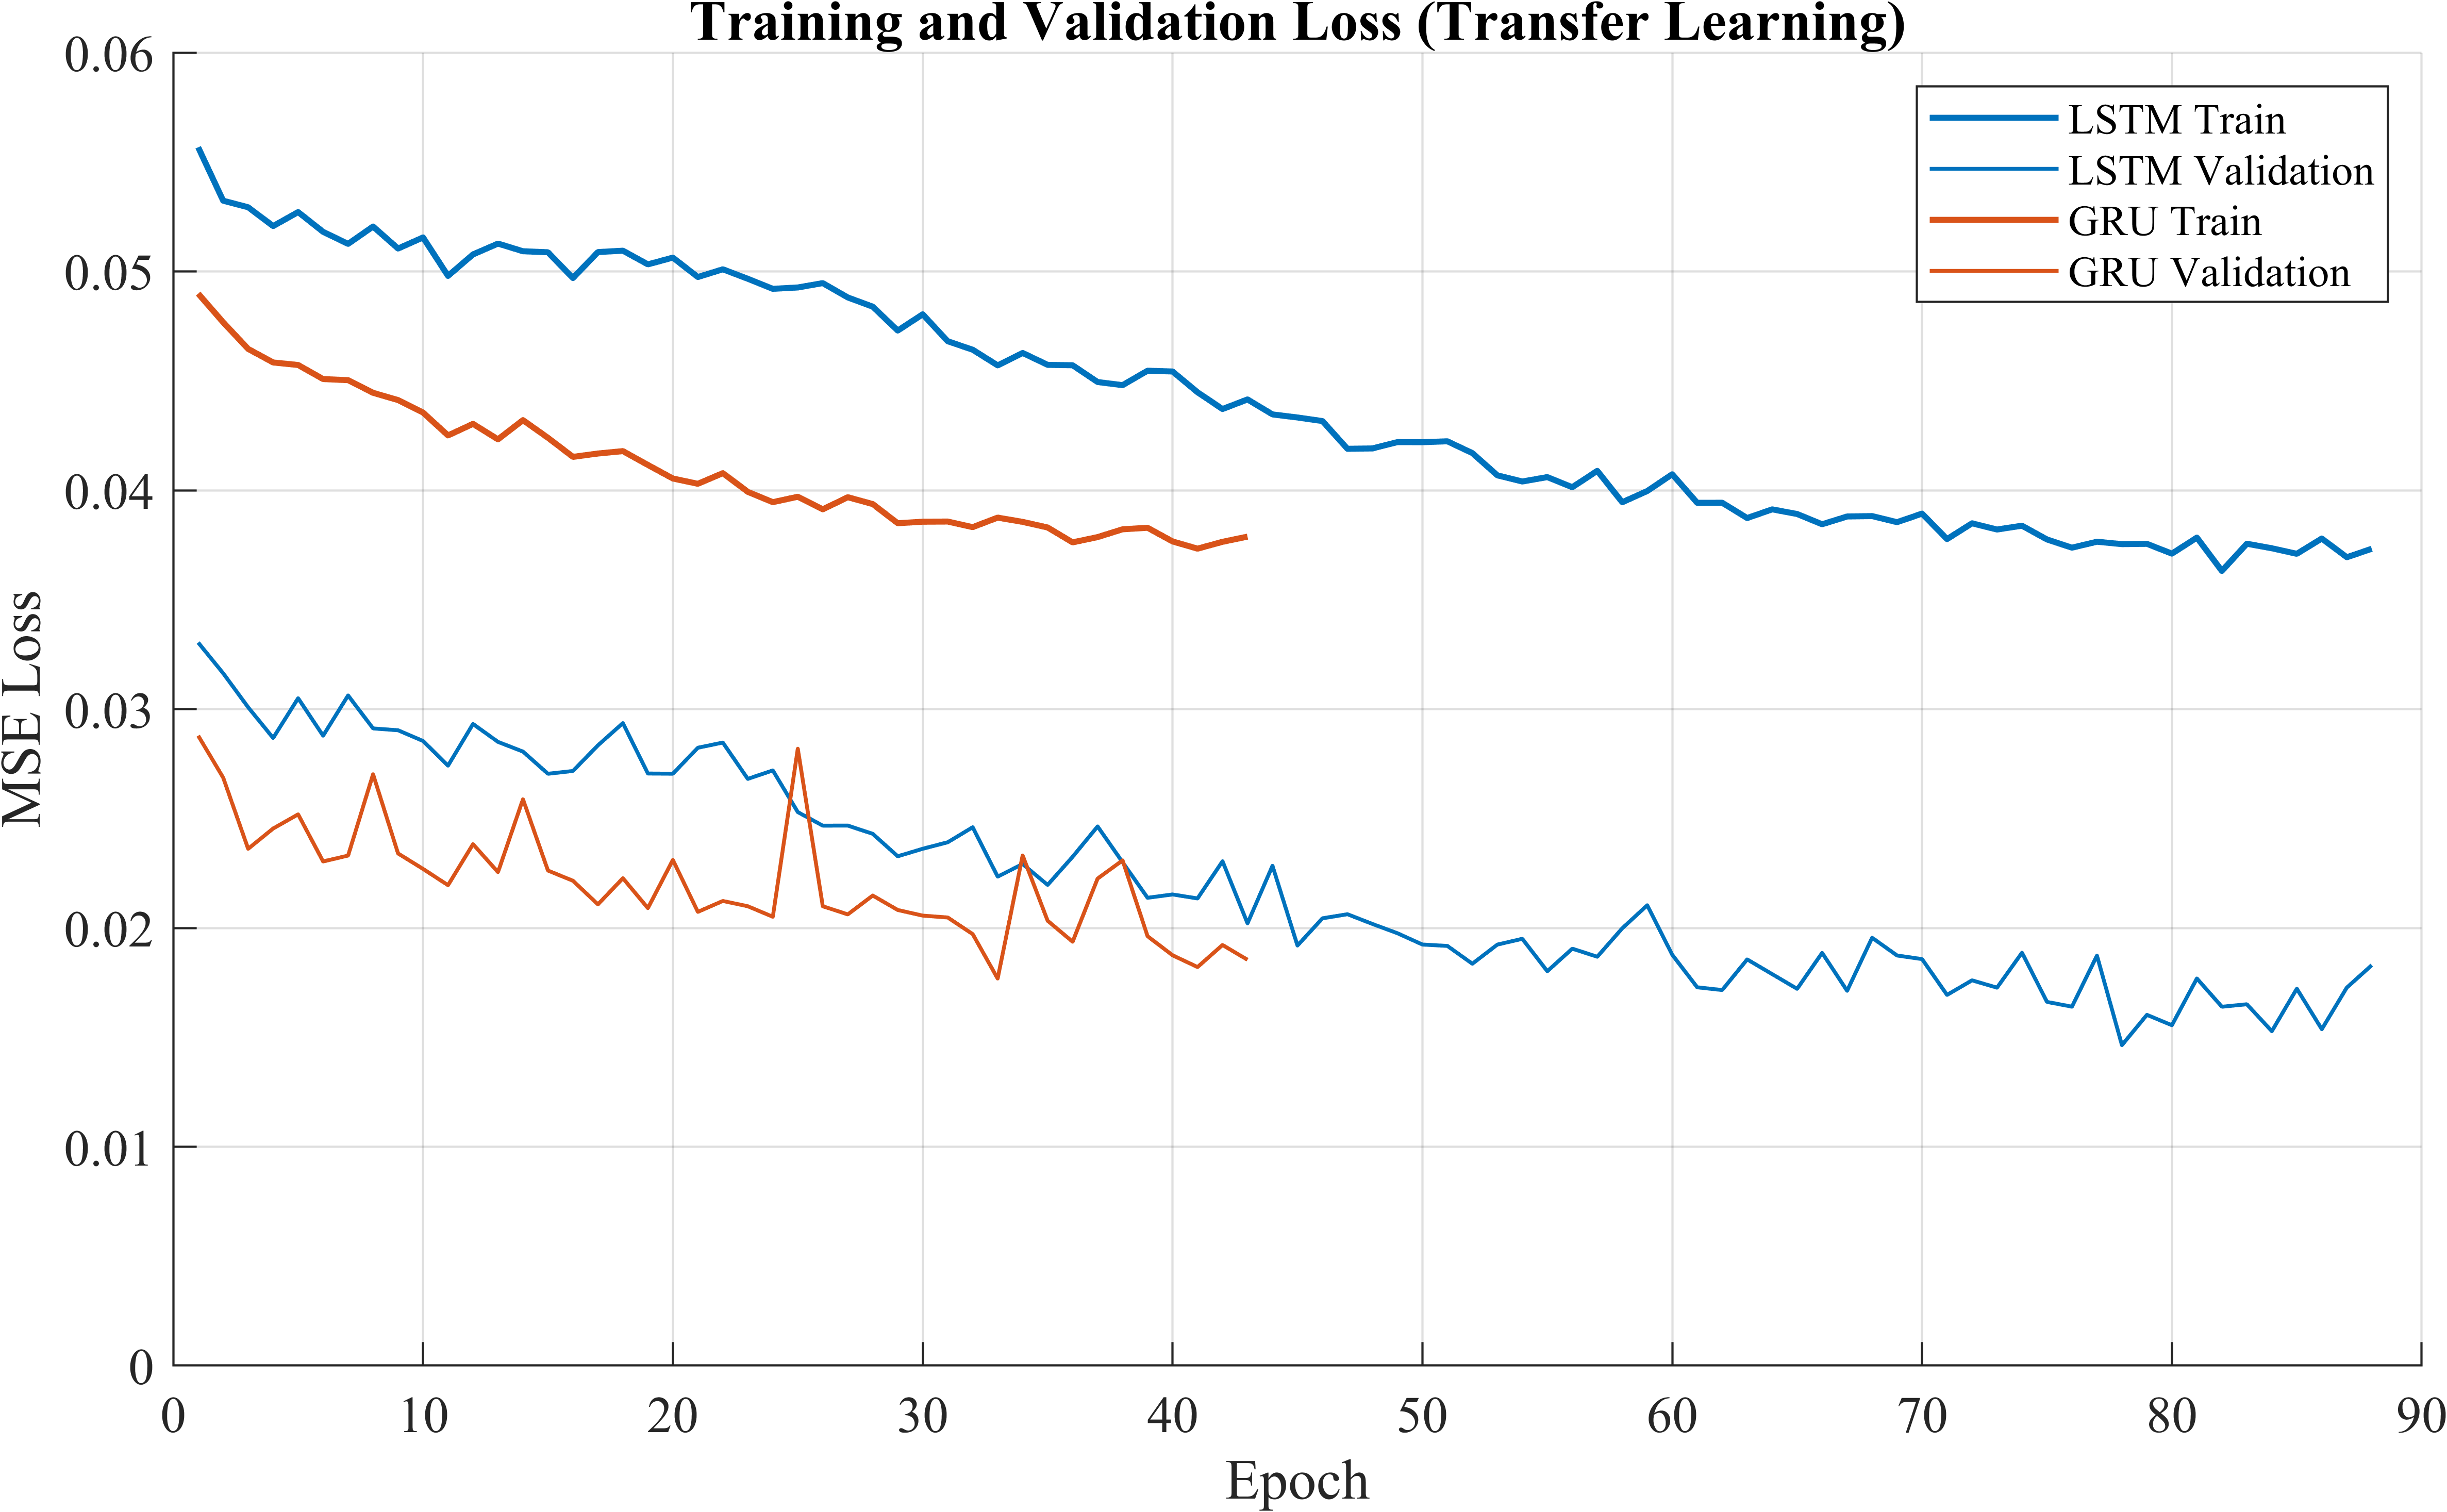
\includegraphics[width=0.8\linewidth]{pics/loss_curve_transfer.png}
    \caption{迁移学习损失曲线对比}
    \vspace{-0.5cm}
\end{figure}
\par{}
测试结果表明，LSTM的Overall MSE、RMSE和MAE均低于GRU；同时，LSTM在四个输出目标上的误差也均小于GRU，说明其迁移后的整体预测精度更高，如图7。
\begin{figure}[H]
    \centering
    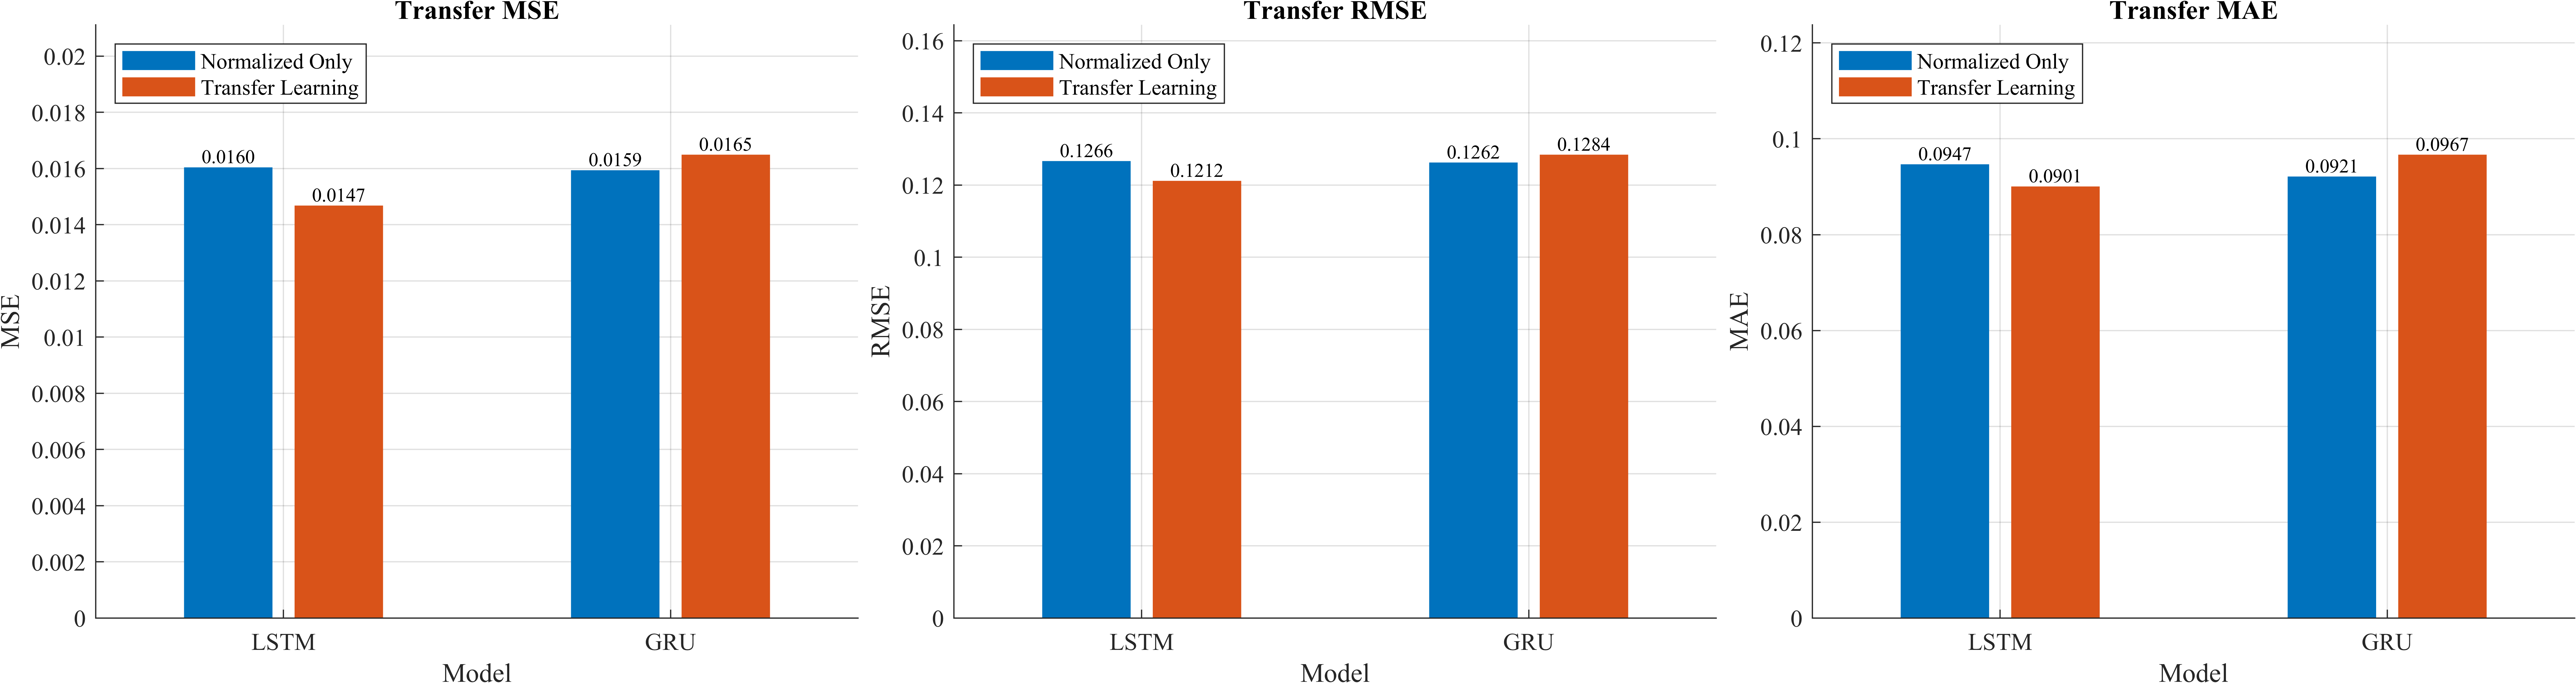
\includegraphics[width=0.98\linewidth]{pics/transfer_learning_metrics_comparison.png}
    \vspace{-0.5cm}
\end{figure}
\newpage{}
\begin{figure}[H]
    \centering
    
\includegraphics[width=0.98\linewidth]{pics/metrics_comparison_transfer.png}
    \caption{两种模型迁移学习效果对比}
    \vspace{-0.5cm}
\end{figure}
\par{}
而对比迁移学习和直接训练所得结果，如图8，对于LSTM，迁移学习后的三个误差指标均低于仅归一化数据上的直接训练结果，说明其在源域中学习到的时序特征对目标域具有一定迁移价值。对于 GRU，迁移学习后的三项误差指标均略高于直接训练结果，表明源域权重并未提升目标域预测性能。这可能是由于 GRU 结构较简洁，直接在目标域数据上训练已经能够较快适应数据分布，而源域权重反而限制了其进一步优化。因此，本实验中迁移学习对LSTM更有效，而对GRU的提升并不明显；迁移学习并不必然提升性能，它是否有效取决于源域和目标域的数据分布差异，以及模型结构对已有权重的利用能力。
\begin{figure}[H]
    \centering
    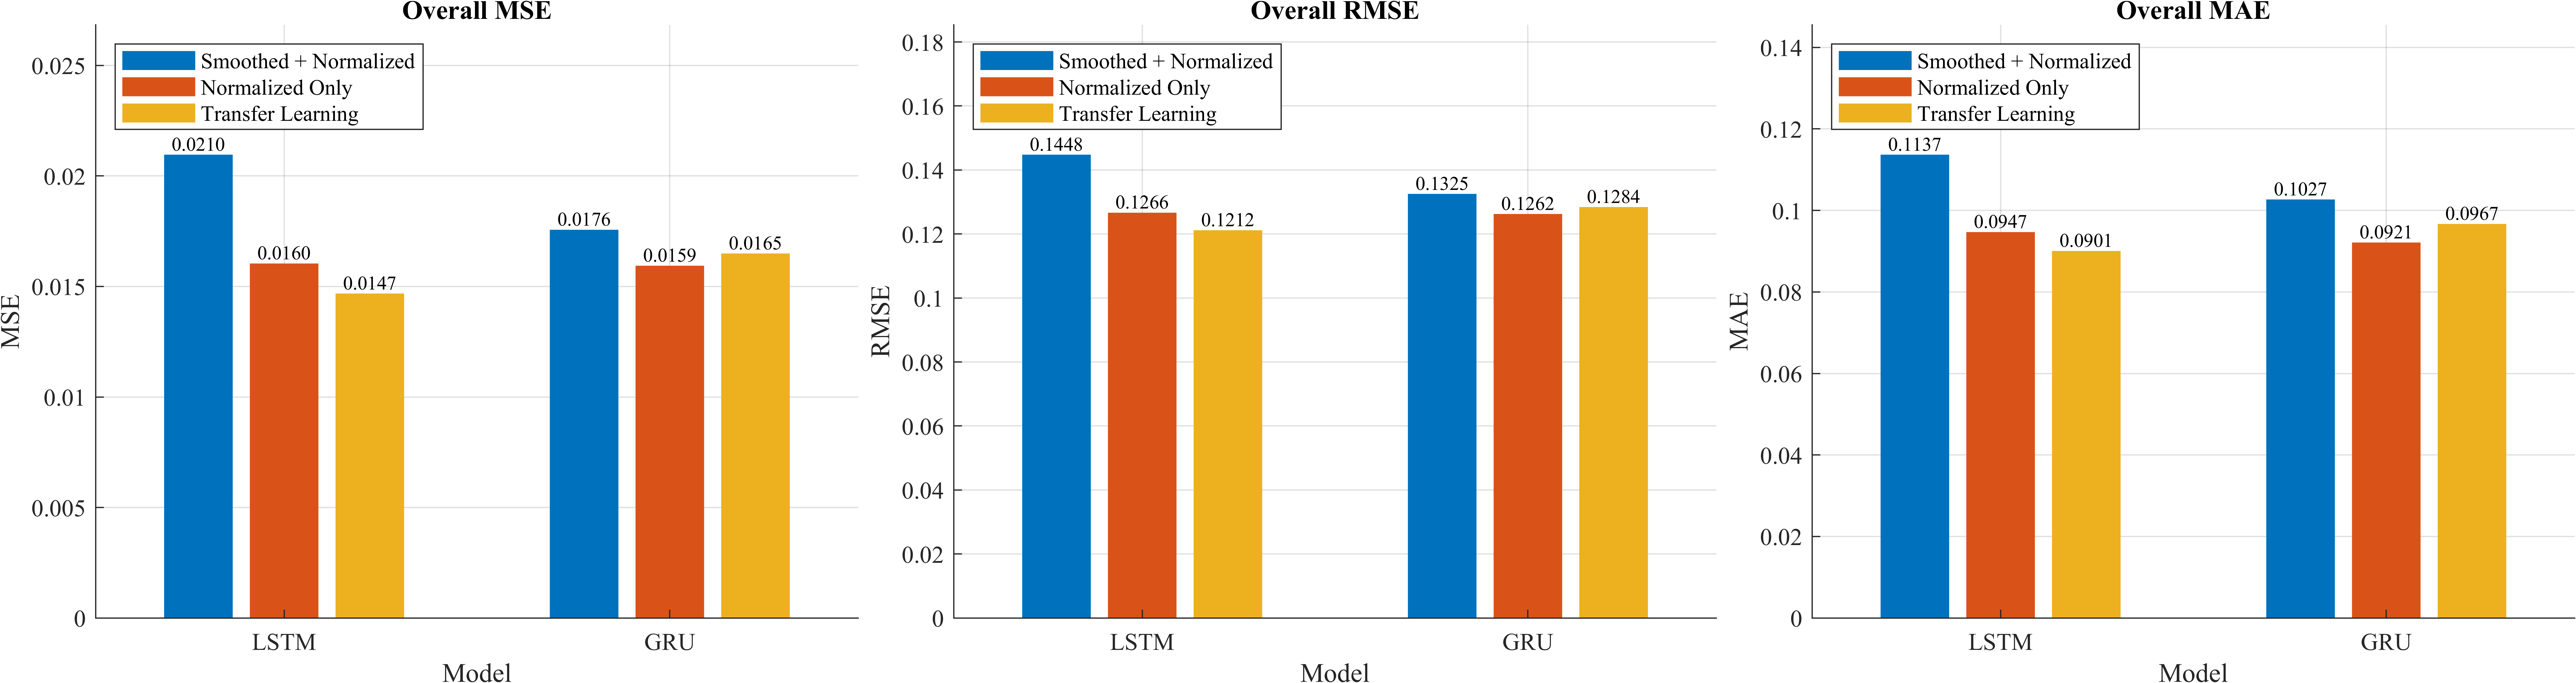
\includegraphics[width=0.98\linewidth]{pics/preprocessing_metrics_comparison_with_transfer.png}
    \caption{迁移训练与直接训练总体指标对比}
    \vspace{-0.5cm}
\end{figure}
\par{}
\quad{}
\par{}
\section{附录：源代码（带注释）}
本项目仓库见\href{https://github.com/XiaoZhefu/RNN-Homework}{\color{blue} https://github.com/XiaoZhefu/RNN-Homework}或附属压缩包文件夹，包含脚本与报告源代码。
\par{}
\quad{}
\par{}
\begin{flushleft}
    \begin{small}
        \begin{thebibliography}{99}
            \bibitem{ref1} PyTorch Contributors. torch.nn.RNN [EB/OL]. PyTorch 2.12 Documentation, 2026[2026-06-05].
            \href{https://docs.pytorch.org/docs/2.12/generated/torch.nn.RNN.html}{\color{blue} https://docs.pytorch.org/docs/2.12/generated/torch.nn.RNN.html}.
            \vspace{-3mm}
            \bibitem{ref2} PyTorch Contributors. torch.nn.LSTM [EB/OL]. PyTorch 2.12 Documentation, 2026[2026-06-05].
            \href{https://docs.pytorch.org/docs/2.12/generated/torch.nn.LSTM.html}{\color{blue} https://docs.pytorch.org/docs/2.12/generated/torch.nn.LSTM.html}.
            \vspace{-3mm}
            \bibitem{ref3} PyTorch Contributors. torch.nn.GRU [EB/OL]. PyTorch 2.12 Documentation, 2026[2026-06-05].
            \href{https://docs.pytorch.org/docs/2.12/generated/torch.nn.GRU.html}{\color{blue} https://docs.pytorch.org/docs/2.12/generated/torch.nn.GRU.html}.
            \vspace{-3mm}
        \end{thebibliography}
    \end{small}
\end{flushleft}



\end{document}
